\documentclass[11pt]{amsart}
\usepackage{geometry,amsmath,amssymb,amsthm,cite,mathtools,float, caption, comment}                % See geometry.pdf to learn the layout options. There are lots.
\usepackage[numbers, sort&compress]{natbib}
\geometry{letterpaper}                   % ... or a4paper or a5paper or ... 
%\geometry{landscape}                % Activate for for rotated page geometry
%\usepackage[parfill]{parskip}    % Activate to begin paragraphs with an empty line rather than an indent
\usepackage{graphicx}
\usepackage{algorithm}
\usepackage[noend]{algpseudocode}
\usepackage{amssymb}
\usepackage{epstopdf}
\usepackage[parfill]{parskip}
\setlength{\parskip}{1ex}
\newtheorem{lemma}{Lemma}
\newtheorem{theorem}{Theorem}
\newtheorem{prop}{Proposition}
\DeclareGraphicsRule{.tif}{png}{.png}{`convert #1 `dirname #1`/`basename #1 .tif`.png}


\title{A compositional model to assess expression changes from
 single-cell RNA-seq data\footnote{Department of Biostatistics and Medical Informatics, UW Madison, Technical Report TR***-v1, February **, 2019.}} 

\author{Xiuyu Ma,  Keegan Korthauer, Christina Kendziorski, and Michael A. Newton}
 
\email{newton@biostat.wisc.edu}
\begin{document}

\begin{abstract}
*blah blah*
\end{abstract}

\maketitle
\section{Introduction}

The ability to measure genome-wide gene expression at single-cell resolution 
has accelerated the pace of biological discovery\cite{scs}.  Overcoming data
analysis challenges caused by the scale and unique variation properties of single-cell
data will surely fuel further advances in immunology\cite{immune}, developmental
biology\cite{dv}, cancer\cite{cancer}, and other areas. 
 Computational tools and statistical methodologies 
created for data of lower-resolution (e.g., bulk RNA-seq) or lower dimension 
(e.g., flow cytometry)  guide our response to 
 the data science demands of new measurement platforms,
but they are not adequate for efficient knowledge discovery in this
rapidly advancing domain\cite{Bacher:2016aa}.

An important feature of single-cell studies that could be leveraged better
statistically is the fact that cells populate distinct, identifiable subtypes
determined by lineage history, epigenetic state, the activity
of various transcriptional programs, or other 
distinguishing factors. Lots of efforts have been made to clustering cells
into different cell subtypes, SC3\cite{sc3}, CIDR\cite{CIDR} and ZIFA\cite{ZIFA}.
We hypothesize that such
subtype information may be usefully injected into various inference procedures in order
to improve their operating characteristics. 

Assessing the magnitude and statistical significance of changes in gene
expression associated with different cellular conditions has been a central
statistical problem in genomics for which new tools specific to
the single-cell RNAseq data structure have been deployed: MAST\cite{ref:MAST},
DESEQ2\cite{ref:Des}, SCDD\cite{ref:scDD}, etc.  These tools respond
to scRNAseq characteristics, such as high prevelance of zero counts and
gene-level multimodality, but none takes explicit advanatage of cellular subtype
information.  We present a simple procedure and supporting theoretical
analyses for this purpose.  A notable technical innovation is a new prior
distribution over pairs of multinomial probability vectors that conveys
both marginal Dirichlet conjugacy as well as
 dependence induced through sharp equalities on aggregated 
 subtype probabilities, which turns out to be key in formulating 
 the posterior probability of changes in expression distributions between conditions.
 
 
Using the proposed compositional model, subtypes inferred from whole genome data 
improve the analysis of gene-level expression.  We utilize the mixture of subtypes to 
characterize transcripts profile and identify differential distributed genes across conditions in an scRNA-seq experiment.
Simulation study suggests that the method provides improved power and precision for identifying differentially distributed genes. 
Performance on empirical data has been investigated through ten previously published experimental data from conquer\cite{ref:Cq}. 
We also obtained asymptotic properties of posterior inference. 

The proposed scDDboost methodology extends scDD\cite{ref:scDD}, which similarly treats expression data within a condition as a statistical mixture.   
The extension provided by the present work is to recognize that this mixture is a mixture over cell subtypes.  
Thus genome-wide data provide information on mixing proportions, thereby providing useful
structural information into each gene-level calculation.   A software implementation of the proposed methodology 
is available in the R package \textsc{scDDboost}, at \verb+http://github.com/wiscstatman/scDDboost/+

\section{Modeling}
\subsection{Data structure, sampling model, and parameters}

In modeling scRNASeq data, we
imagine that each cell $c$ falls into one of $K>1$ classes, which we think of as
subtypes or subpopulations of cells. For notation, $z_c=k$ means that cell $c$ happens to be of subtype $k$, with the vector $z=(z_c)$ recording
the states of all sampled cells.  Knowledge of this class structure
 prior to measurement is not required, as it will be inferred as necessary from
 available genomic data.   We expect that cells arise from multiple
experimental conditions, such as by treatment-control status or some other factors
 measured at the cell level, but we present our development for the special
case of two conditions.  Notationally, $y=(y_c)$ records the experimental condition, say $y_c=1$ or $y_c=2$ initially:
extensions to multiple conditions are discussed in section 6. Let's say condition $j$ measures $n_j=\sum_{c} 1[y_c=j]$ cells,  and
in total we have $n=n_1+n_2$ cells in the analysis.  Further let 
\begin{eqnarray}
\label{eq:counts}
t^j_k = t^j_k(y,z) = \sum_c 1[y_c=j, z_c=k] 
\end{eqnarray}
denote the number of cells of subtype $k$ in condition $j$;
we infer something about these counts using genome-wide data.  As for molecular data, the 
normalized expression of gene $g$ in cell $c$, say $X_{g,c}$, is one entry
in a typically large {\sc{genes}} by {\sc{cells}} data matrix $X$.  Thus, the data structure entails an expression matrix
$X$, a treatment label vector $y$, and a vector $z$ of latent subtype labels.


We treat subtype counts in the two conditions,  $t^1 = (t^1_1, t^1_2, \cdots, t^1_K )$ and 
$t^2 = (t^2_1, t^2_2, \cdots, t^2_K)$,  as independent multinomial
vectors, reflecting the experimental design.  Explicitly,
\begin{eqnarray}
\label{eq:mult}
t^1| y \sim \text{Multinomial}_K( n_1, \phi ) \quad {\mbox {\rm and}} \quad
t^2| y \sim \text{Multinomial}_K( n_2, \psi )
\end{eqnarray}
for probability vectors 
$\phi = (\phi_1, \phi_2, \cdots, \phi_K)$ and 
 $\psi = ( \psi_1, \psi_2, \cdots, \psi_K)$ that characterize the populations of
cells from which the $n$ observed cells are sampled.  This follows from the more basic 
sampling model:
$P(z_c=k|y_c=1) = \phi_k$ and $P(z_c=k| y_c =2 ) = \psi_k.$

Our working hypothesis, referred to as the {\em compositional model},  is that any differences in the distribution of expression $X_{g,c}$ 
between $y_c=1$ and $y_c=2$ (i.e., any condition effects) are attributable 
to differences between the conditions 
in the underlying composition of cell types; i.e.,
owing to $\phi \neq \psi$.  We reckon that cells of any given subtype $k$ will
present data according to a distribution reflecting technical 
and biological variation specific to that class of cells, regardless of the 
condition the cell finds itself in.   Some care is needed in this, as an overly
broad cell subtype (e.g., {\em epithelial cells}) could have
further subtypes that show differential response to some treatment, for example,
and so cellular condition (treatment) would then affect the distribution of 
expression data within the subtype, which is contrary to our working hypothesis.
Were that the case,  we could have refined the subtype definition to allow a greater
number of population classes $K$ in order to mitigate the problem of within-subtype 
heterogeneity. A  risk in this approach is that $K$ could approach $n$, as if  
every cell were  its own subtype.  We find, however,
that data sets often encountered do not display this theoretical phenomenon
when considering a broad class of within-subtype expression distributions.
We revisit the issue in discussion section, but for now proceed assuming 
that cellular condition affects the composition of subtypes but not the distribution of expression
within a subtype.

Within the compositional model, let $f_{g,k}$ denote the sampling distribution
of expression measurement $X_{g,c}$ assuming that cell $c$ is from subtype $k$.
Then for the two cellular conditions, and at some expression level $x$, 
the marginal distributions over subtypes are finite mixtures:
\begin{eqnarray*}
f_g^1(x) = \sum_{k=1}^K \phi_k f_{g,k} (x) \quad {\mbox {\rm and}} \quad
f_g^2(x) = \sum_{k=1}^K \psi_k f_{g,k} (x).
\end{eqnarray*}
In other words,  $X_{g,c} |[ y_c=j]  \sim f_g^j$  and $X_{g,c} |[ z_c=k, y_c=j] \sim f_{g,k}$.

We say that gene $g$ is {\em differentially distributed}, denote ${\rm DD}_g$ and indicated
$f_g^1 \neq f_g^2$,
if $f_g^1(x) \neq f_g^2(x)$ for some $x$, and otherwise it is equivalently distributed
(${\rm ED}_g$). Motivated by findings from bulk RNAseq data analysis, we further
set each $f_{g,k}$ to have a a negative-binomial form, say with mean $\mu_{g,k}$
and shape parameter $\alpha_g$ (\cite{ref:Leng};\cite{DES};\cite{ref:Des}). 
This choice proves to be effective in our numerical experiments though it is 
not critical to the modeling formulation.  The use of mixtures per gene has proven
useful in related model-based approaches (e.g., Finak {\em et al.} 2015; McDavid {\em et al.} 2016;
Huang {\em et al.} 2018).
Our perspective is that  genome-wide data may usefully inform the  mixing proportions.

We seek methodology to prioritize genes for evidence
of ${\rm DD}_g$.  Interestingly, even if we have evidence for condition effects
on the subtype frequencies, it does not follow that a given
gene will have $f^1_g \neq f^2_g$; that depends on whether or not the subtypes
show the right pattern of {\em differential expression} at $g$, to use the 
standard terminology from bulk RNAseq.  For example, if two subtypes have 
different frequencies between the two conditions ($\phi_1 \neq \psi_1$ and 
 $\phi_2 \neq \psi_2$) but the same aggregate frequency
($\phi_1+\phi_2 = \psi_1 + \psi_2$),  and also  if $\mu_{g,1} = \mu_{g,2}$
then, other things being equal, $f^1_g = f^2_g$ even though $\phi \neq \psi$.
Simply, a gene that does not distinguish two subtypes will also not distinguish
the cellular conditions if those subtypes appear in the same aggregate frequency
in the two conditions, regardless of changes in the individual subtype 
frequencies. (A second, pedagogical example is presented in the Supplementary
Material file.)  We formalize the idea in order that our methodology
has the necessary functionality.  To do so,  first consider the parameter space 
$\Theta = \{ \theta=(\phi, \psi,\mu, \sigma)  \}$,
where $\phi=(\phi_1, \phi_2, \cdots, \phi_K)$ and $\psi=(\psi_1, \psi_2, \cdots, \psi_K)$ 
are as before, where $\mu = \{ \mu_{g,k} \}$ holds  all the subtype-and-gene-specific expected
values, and where $\sigma = \{ \sigma_g \}$ holds all the gene-specific negative-binomial
shape parameters.  Critical to our construction are special subsets of $\Theta$ corresponding
to partitions of the $K$ cell subtypes.  A single partition, say $\pi$, is a set of
mutually exclusive and exhaustive blocks, $b$, say, each a subset of $\{1, 2, 
\cdots, K\}$, and we write $\pi = \{ b \}$.  Of course,
the set $\Pi$ containing all partitions $\pi$ of $\{1,2, \cdots, K\}$
 has cardinality that grows rapidly with $K$. 
 We carry along an example
involving $K=7$ cell types, and one three-block partition taken
from the set of 877 possible partitions of $\{1, 2, \cdots, 7\}$ (Figure 1).

\begin{figure}[h!]
  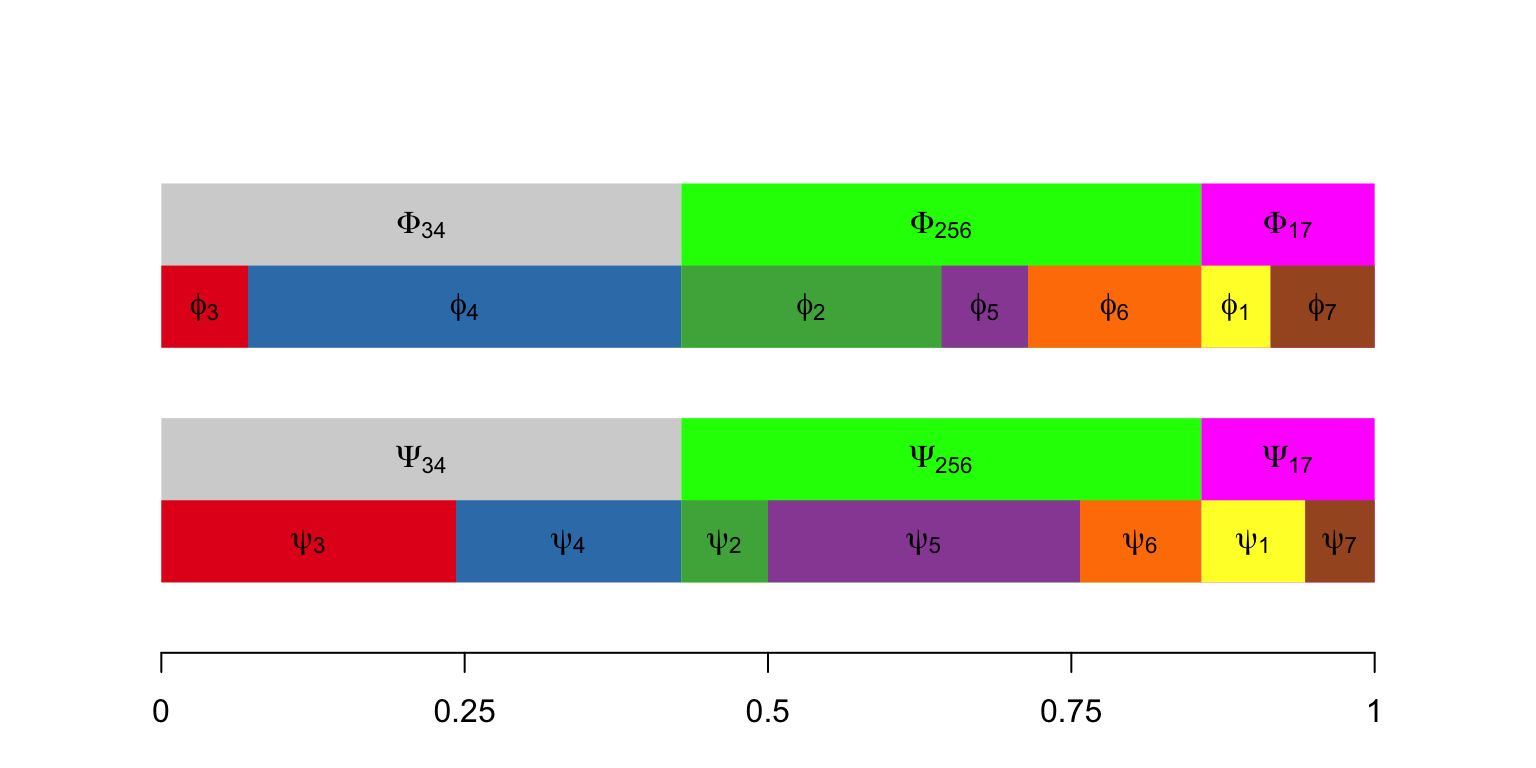
\includegraphics[width=\linewidth]{Figs/schematic-1.png}
  \caption{Proportions of $K=7$ cellular subtypes in different conditions. 
 Aggregated proportions of subtypes 3 and 4, subtypes 2, 5, and 6, and subtypes 1, and 7 
 remain same across conditions, while individual subtype frequencies change.  }
  \label{fig:1}
\end{figure}

%% Xiuyu, the alternative figure you had offered gives the suggestion that blocks of the
%% partition may need to be contiguous classes, which is not so...; with some other
%% stylistic differences, I decided to go back to the original; I realize your simulation
%% was not based on this one, but maybe that's ok


For any partition $\pi=\{b\}$, consider aggregate subtype frequencies
\begin{eqnarray*}
\Phi_b = \sum_{k\in b} \phi_k \quad {\mbox {\rm  and}} \quad 
 \Psi_b = \sum_{k\in b} \psi_k,
\end{eqnarray*}
and extend the notation, allowing vectors $\Phi_\pi = \{ \Phi_b: b \in \pi \}$ and similarly
for $\Psi_\pi$. Recall the partial ordering of partitions based on refinement, and note that
as long as $\pi$ is not the most refined partition (every cell type its own block),
then the mapping from $( \phi, \psi )$ to $( \Phi_\pi, \Psi_\pi)$ is many-to-one.
Further, define sets
\begin{eqnarray}
\label{eq:asets}
A_\pi = \{ \theta\in \Theta: \; \Phi_b = \Psi_b  \, \forall b \in \pi \}.
\end{eqnarray}
and
\begin{eqnarray}
\label{eq:msets}
M_{g,\pi} = \{ \theta \in \Theta: \; \mu_{g,k} = \mu_{g,k'} \iff k,k' \in b, b \in \pi \}.
\end{eqnarray}
Under $A_\pi$ there are constraints on cell subtype frequencies; under $M_{g,\pi}$ there is 
equivalence in the gene-level distribution of expression between certain subtypes.
These sets are precisely the
structures needed to address differential distribution DD$_g$ (and
it complement, equivalent distribution, ${\rm ED}_g$) at a given gene
$g$, since:

\begin{theorem}  Let $C_{g,\pi} = A_\pi\cap M_{g, \pi}$.  For distinct 
partitions $\pi_1,\pi_2$, $C_{g,\pi_1} \cap C_{g,\pi_2} = \emptyset$. Further,
 at any gene $g$, equivalent distribution is
\begin{eqnarray*}
{\rm{ED}}_g = \bigcup_{\pi \in \Pi} C_{g,\pi}.
\end{eqnarray*}
\end{theorem}
With additional 
probability structure on the parameter space,  we immediately obtain from Theorem~1 
a formula for local false discovery rates:
\begin{align}
\label{eq:lfdr}
1-P(\text{DD}_g|X,y) = 
 P(\text{ED}_g|X,y) = \sum_{\pi \in \Pi} P\left(A_\pi \cap M_{g,\pi} |X,y \right).
\end{align}
Such local false discovery rates are important empirical Bayesian 
statistics in large-scale testing (e.g., Efron, 2007; Muralidharan, 2010; Newton 
{\em et al.} 2004).
The partition representation guides construction of a prior distribution (Section 3.1) and a 
model-based method (Section 2.3) for scoring  differential distribution.   Setting the stage, 
Figure~2 shows the dependency structure of 
the proposed compositional model and the partition-reliant prior specification.

\begin{figure}[h!]
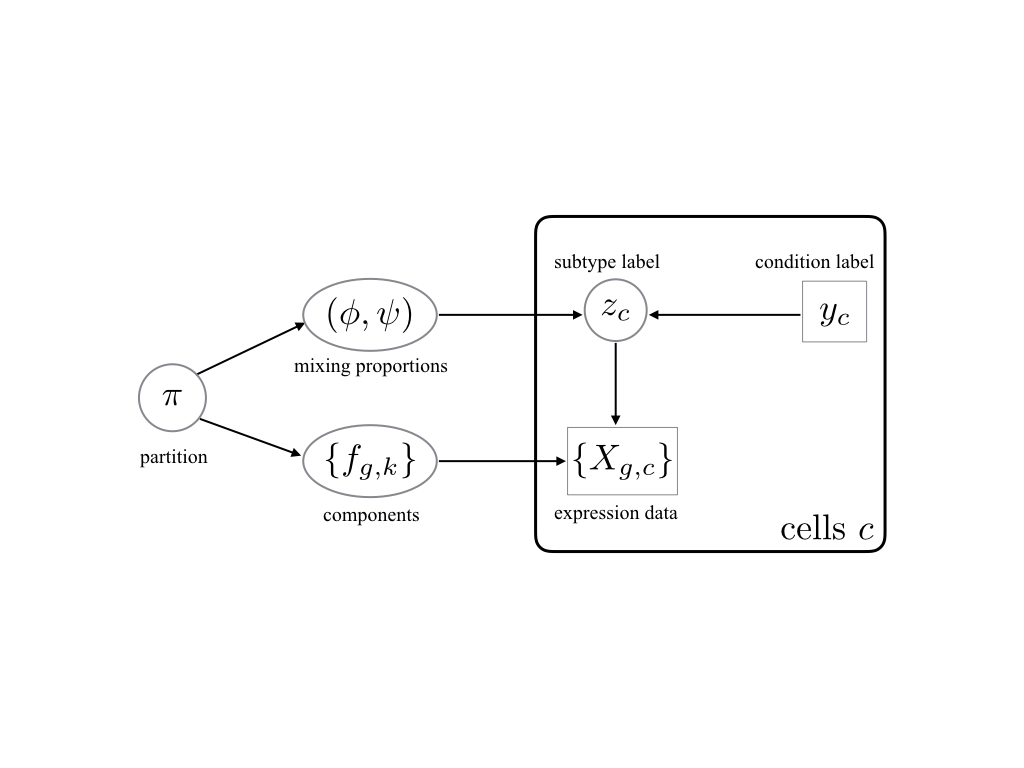
\includegraphics[trim={4cm 6cm 4cm 6cm}, clip, width=5in]{Figs/dag.png}
  \caption{Directed acyclic graph structure of compositional 
model and partition-reliant prior. The plate on the right side indicates i.i.d.
copies over cells $c$, conditionally on mixing proportions and mixing components.
 Observed data are indicated in rectangles/squares, and unobserved variables
are in circles/ovals. }
  \label{fig:2}
\end{figure}

Key to computing the gene-specific 
local false discovery rate $P(\text{ED}_g|X,y)$ is
evaluating probabilities $P\left(A_\pi \cap M_{g,\pi} |X,y \right)$ for
any subtype partition $\pi$ and gene $g$.
The dependence structure (Figure~2) implies a useful reduction of this
quantity, at least conditionally upon subtype labels $z=(z_c)$.

\begin{theorem}  
$  P\left(A_\pi \cap M_{g,\pi} |X,y,z \right) 
  =  P\left(A_\pi |y,z \right) \, 
                      P\left(M_{g,\pi}| X,z \right).  $
\end{theorem}

In what follows, we develop the  modeling and computational elements necessary  to efficiently evaluate inference summaries~(\ref{eq:lfdr}) taking advantage of 
Theorems~1 and~2.  Roughly, the methodological idea is that subtype labels $z$
have relatively low uncertainty, and may be estimated from genome-wide 
clustering of cells in the absence of condition information $y$. The modest bit of uncertainty in $z$
we handle through a computationally efficient randomized clustering scheme.
 Theorem~2 indicates that our computational task then separates into
two parts given $z$.  On one hand, cell subtype frequencies 
combine with condition labels to give
$P\left(A_\pi |y,z \right)$. Then gene-level data
locally drive the posterior probabilities $P\left(M_{g,\pi}| X,z \right)$ that
measure differential expression between subtypes. 
Essentially, the model provides a specific form of information 
sharing between genes  that leverages the compositional structure of single-cell 
data in order to sharpen our assessments of between-condition expression changes. 


\subsection{Method structure and clustering}

We leverage the extensive research on how to cluster cells into subtypes using scRNA-seq data (e.g., 
 SC3\cite{sc3}, CIDR\cite{CIDR}, and ZIFA\cite{ZIFA}).   We propose clustering on the full set
of profiles in a way that is blind to the condition label vector $y$, in order to have as many cells as possible
to inform the subtype structure.  We investigated several clustering schemes in numerical experiments and allow 
flexibility in this choice within the \textsc{scDDboost} software. 
Associating clusters with subtype labels $\hat z_c$  estimates
the actual subtypes $z_c$, and prepares us to use Theorems~1 and~2 in order to compute separate
posterior probabilities $P(A_\pi|y, \hat z)$ and $P(M_{g, \pi}| X, \hat z)$ that are necessary for scoring
differential distribution. The first probability concerns patterns of cell counts over subtypes in the two conditions,
and has a convenient closed form within the {\em double Dirichlet} model introduced in Section~3.1.
The second probability concerns patterns of changes in expected expression levels among subtypes, and this is
also conveniently computed for negative-binomial counts using \textsc{EBSeq} \cite{ref:Leng}. For completeness
we review in Appendix~A the empirical Bayes model underlying \textsc{EBSeq}.  Algorithm~\ref{alg:scDDcore}
summarizes how these elements combine to get the posterior probability of differential distribution per gene,
conditional on an estimate of the subtype labels.


%Our approach take transcripts processed by normalizing methods (e.g. SCnorm \cite{ref:Rhonda}). 
%The workflow contains two parts, classify cells into subtypes and posterior inference on distributional change. In the first part, recall subtype is a group of cells with distributions of transcripts that are specific to this group, regardless which condition the cells is from. Thus classification process is blind to conditions and can be done by clustering upon similarities between cells(supplementary material). 

\begin{algorithm}
\caption{\textsc{scDDBoost-core}}\label{alg:scDDcore}
\raggedright\hspace*{\algorithmicindent} \textbf{Input}: \begin{list}{}{}
 \item \textsc{genes} by \textsc{cells} expression data matrix $X=(X_{g,c})$
 \item  cell condition labels $y=(y_c)$ 
 \item  cell subtype labels (estimated)  $\hat z=(\hat z_c)$
 \end{list}
\hspace*{\algorithmicindent} 
\textbf{Output}:  posterior probabilities of differential distribution from estimated subtypes
\begin{algorithmic}[1]
\Procedure{scDDBoost-core}{$X,y,\hat z$}
 \item  number of cell subtypes $K = \rm{length}( \rm{unique}( \hat z ) )$  
\State subtype differential expression: $\forall g,\pi$ compute  $P(M_{g,\pi} | X, \hat z)$ using EBSeq\cite{ref:Leng}
\State cell frequency changes: $\forall \pi$ compute  $P(A_\pi | y, \hat z)$ using Double Dirichlet model 
\State posterior probability: $\forall g,  \, P(\text{ED}_g | X, y, \hat z)\gets \underset{\pi}{\sum}P(M_{g,\pi} | X, \hat z) \,
 P(A_\pi | y, \hat z)$
\State \textbf{return} $\forall g, \, P(\text{DD}_g |X, y, \hat z)=1-P(\text{ED}_g| X,y, \hat z)$
\EndProcedure
\end{algorithmic}
\end{algorithm}



%%One advantage of our approach is that the posterior inference can be incorporate with different clustering methods. With the development of technology, clustering methods taking care of newly discovered characteristic of scRNA seq data (e.g. SC3\cite{sc3}, CIDR\cite{CIDR} and ZIFA\cite{ZIFA}) could be substituted with our default one. No matter what clustering method is used, we estimate the mixture structure utilizing the whole genome information rather than estimating a gene specific mixture structure solely using information of that gene. Due to this reason, our model is more capable of capturing characteristic of scRNA seq data than scDD and we name our approach \textsc{scDDboost}. 

We invoke $K-$medoids (\cite{kmedoids}) 
as the default clustering method in \textsc{scDDboost}, and customize the cell-cell distance by integrating two measures.  
The first assembles gene-level information by cluster-based-similarity partitioning (\cite{ref:cspa}).
 Separately at each gene,   modal clustering (\cite{ref:dahl} and Appendix B) partitions the cells, and
then we define dissimilarity between cells as the proportion of genes at which the cells are assigned to different clusters. 
A second measure defines dissimilarity by one minus the 
Pearson correlation between cells, which is computationally inexpensive,
less sensitive to outliers than Euclidean distance, and effective at detecting cellular clusters in scRNA-seq(\cite{Cor}).
 We combine the two measures by a weighted average, 
with  $w_C = \frac{\sigma_C}{\sigma_C + \sigma_P}$ and $w_P = 1 - w_C$. where $w_C,\sigma_C, w_P, \sigma_P$ are the weights and standard deviations of cluster based distance and Pearson correlation distance accordingly.   
The resulting distance matrix is $D=\left( d_{i,j} \right)$. 

Any clustering method  entails classification errors, and so $\hat z_c \neq z_c$ for some cells. To mitigate
the effects of this uncertainty, \textsc{scDDboost} averages output probabilities from \textsc{scDDboost-core} over
randomized clusterings $\hat z^*$.  These are not uniformly random, but rather are generated by applying $K-$medoids
to a randomized distance matrix $D^*=\left( d_{i,j}\times w_{i,j}\right)$, 
where $w_{i,j}$ are  unit mean, non-negative weights
$w_{i,j} = 1/( e_i + e_j )$, and where $( e_i) $ are independent and identically Gamma$(\hat a, \hat b)$ distributed
deviates for hyper-parameters $(\hat a, \hat b)$ derived from $D$.   We argue (Appendix C) that the distribution of
clusterings induced by this simple scheme approximates a Bayesian posterior analysis.   Pseudo-code for the resulting
\textsc{scDDboost} is in Algorithm~\ref{alg:scDDboost}.

%%Computations become more intensive the larger is the number $K$ of cell subtypes.   We observe that gene-specific
%%posterior probabilities of differential distribution stabilize when $K$ is sufficiently large, and we use changes
%%in these profiles to set $K$.
In order to determine the number of clusters, we consider the change of {\em validity} = $\frac{\textbf{intra}}{\textbf{inter}}$ defined in \cite{selK}, where $\textbf{intra} = \frac{1}{N}\overset{K}{\underset{i = 1}{\Sigma}}\underset{x \in C_i}{\Sigma} ||x - z_i||^2$, $\textbf{inter} = mean( || z_i - z_j||^2), i = 1,2,...,K-1. j = i+1,...,K$ and $z_i$ is the center(medoids) of cluster $i$. $\textbf{intra}$ is the average of distance of a point to its corresponding cluster center, which measures the compactness of clusters. We made a small change here, in original paper $\textbf{inter}$ was defined as minimum distance between medoids, we use average instead for the purpose of getting a smoother quantity. $\textbf{inter}$ is the average distance of two cluster centers, which measures the separation between clusters. We want to have a small intra-cluster distance and a big inter-cluster distance, consequently we wnat to minimize the {\em validity}. From empirical study, we constantly observe a monotone decreasing relation between number of clusters and {\em validity}. However this quantity stabilize when $K$ is sufficiently large. The stopping rule for searching $K$ is when $|validity_{K} - min(validity_K) | < \epsilon$ is satisfied. 

%%Although there are various options for clustering methods, none of them guarantee the accuracy and posterior inference of differential distributed genes can be sensitive to the initial partition. Here we provide a method to make our inferences robust to partitions. Given number of subtypes $K$, the final posterior probabilities is obtained by averaging results from iterative run of \textsc{scDDboost-core}  with randomly generated subtype labels $z^*$. Taking account of information contained in $D = dist(X)$ , instead of purely random assigning subtype labels, we generate the distance matrices of cells $D^*$ by dividing weights to the original one and assign labels based on $D^*$. Specifically,  we random sample a noise vector $e$ with length equal to number of cells and components are i.i.d. gamma distributed,  then constructing the weighting matrix $W$ by $W_{i,j} = e_i + e_j$ and random distance matrix is obtained by $D^* = D /  W$(division is performed componentwisely).  The choice of gamma distributed weights and dividing transformation is to matched the probability of two units classified into the same group under random weighting to bayesian framework (supplementary material). 


In simulations, 
we observed that averaged adjusted Rand index as well as Rand index of mode of partitions based on randomized distance matrices is higher (better estimation) than that of partition based on original distance matrix (Supplementary Material, **?**). 
{\em MAN to XM: please clarify}


\subsection{Double Dirichlet Mixture (DDM)}


%** ON THE PRIOR INDEPENDENCE**
%This expresses the idea that  subtype proportions $(\phi,\psi)$ are
%uninformative about the mean expression levels   $\{\mu_{g,i}\}$). Under this assumption:
%**


Here we describe the partition-reliant prior $p(\phi,\psi)$ indicated in~Figure~2 and derive an explicit
formula for $P(A_\pi|y,z)$.   We lose no generality here by defining
$A_\pi = \{ (\phi,\psi): \Phi_b = \Psi_b \;  \forall b \in \pi \}$, rather than as a subset of the full
parameter space as in~(\ref{eq:asets}).   Each $A_\pi$ is closed and convex subset of the product space
holding all possible pairs of length-$K$ probability vectors.

We propose a spike-slab-style mixture prior with the following form:
\begin{eqnarray}
\label{eq:ddmix}
p(\phi,\psi) = \sum_{\pi \in \Pi} \omega_\pi  \, p_\pi(\phi,\psi ).
\end{eqnarray} 
Each mixture component $p_\pi(\phi,\psi)$ has support $A_\pi$;  
the mixing proportions $\omega_\pi$ are any non-negative constants summing to one. 
To specify component $p_\pi$,  notice that on $A_\pi$ there is a 1-1 correspondence between pairs $(\phi, \psi)$ and 
parameter states:
\begin{eqnarray}
\label{eq:onetoone}
 \left\{ (\tilde \phi_b, \tilde \psi_b, \Phi_b), \; \forall b \in \pi \right\}, 
\end{eqnarray}
where
\begin{eqnarray*}
\tilde{\phi}_b = \frac{\phi_b}{\Phi_b}, \quad \tilde{\psi}_b = \frac{\psi_b}{\Psi_b}, \quad 
{\mbox {\rm and}} \quad \Phi_b = \sum_{k \in b} \phi_k = \sum_{k \in b} \psi_k = \Psi_b.
\end{eqnarray*}
For example, $\tilde{\phi}_b$ is a vector of conditional probabilities for each subtype given that a cell
from the first condition is one of the subtypes in $b$. 


We introduce hyperparameters
$\alpha^1_k, \alpha^2_k>0$ for each subtype $k$, and set 
$\beta_b = \sum_{k \in b}\left( \alpha^1_k + \alpha^2_k \right)$ for any possible block $b$.
Extending notation, let $\alpha_b^j$ be the vector of $\alpha_k^j$
for $k\in b$, $\beta_\pi$ be the vector of $\beta_b$ for $b \in \pi$, $\phi_b$ and $\psi_b$ be vectors
of $\phi_k$ and $\psi_k$, respectively, for $k\in b$, and $\Phi_\pi$ and $\Psi_\pi$ be the vectors
of $\Phi_b$ and $\Psi_b$ for $b \in \pi$.  The proposed double-Dirichlet component 
$p_\pi$ is determined in the transformed scale by assuming $\Psi_\pi = \Phi_\pi$ and further:
\begin{eqnarray}
\label{eq:doubledir}
\Phi_\pi  &\sim& \text{Dirichet}_{N(\pi)}[   \beta_\pi   ]  \\ \nonumber
\tilde \phi_b  &\sim & \text{Dirichlet}_{N(b)}[ \alpha_b^1 ] \qquad \forall b \in \pi \\ \nonumber
\tilde \psi_b  &\sim & \text{Dirichlet}_{N(b)}[ \alpha_b^2 ] \qquad \forall b \in \pi 
\end{eqnarray}
where $N(\pi)$ is the number of blocks in $\pi$ and $N(b)$ is the number of subtypes in $b$, and
where all random vectors in~(\ref{eq:doubledir}) are mutually independent.  
Mixing over $\pi$ as in~(\ref{eq:ddmix}), we write
$(\phi,\psi) \sim {\mbox {\rm DDM}}\left[ \omega=(\omega_\pi),
\alpha^1=(\alpha^1_k), \alpha^2 = (\alpha^2_k) \right].$


We record some properties of the component distributions $p_\pi$:
%%using the well-known Dirichlet-multinomial conjugacy and the Dirichlet collapsing property (\cite{ref:Dickey}). 

\noindent
{\bf Property 1:}  In $p_\pi(\phi,\psi)$, $\psi$ and $\phi$ are dependent, unless $\pi$ is the null 
partition in which all subtypes constitute a single block.

%\noindent
%{\bf Property 2:}  If $\alpha^1=\alpha^2$, then both $\phi$ and $\psi$ are marginally distributed
%as Dirichlet$_K(\alpha^1)$.  

\noindent
{\bf Property 2:} With $k \in b$, marginal means are:
\begin{eqnarray*}
E_\pi\left( \phi_k \right ) = \frac{ \alpha^1_k }{ \sum_{k' \in b} \alpha^1_{k'} } \,
		\frac{ \beta_b }{ \sum_{b' \in \pi} \beta_{b'} } \quad {\mbox {\rm and}} \quad
E_\pi\left( \psi_k \right ) = \frac{ \alpha^2_k }{ \sum_{k' \in b} \alpha^2_{k'} }  \,
		\frac{ \beta_b }{ \sum_{b' \in \pi} \beta_{b'} } .
\end{eqnarray*}

Recall from~(\ref{eq:counts}) the vectors $t^1$ and $t^2$ holding
counts  of cells in each subtype in each condition, computed from $y$ and $z$.  Relative to a block $b \in \pi$, 
let $t^j_b = \sum_{k\in b} t^j_k$, for cell conditions $j=1,2$, and,
let $t^j_\pi$ be the vector of these counts over $b \in \pi$.   The following properties refer to
marginal distributions in which $(\phi,\psi)$ have been integrated out of the joint
distribution involving~(\ref{eq:mult}) and the component $p_\pi$.

\noindent
{\bf Property 3:}  $t^1$ and $t^2$ are conditionally independent given $y$, $t^1_\pi$ and $t^2_\pi$.

\noindent
{\bf Property 4:}  For $j=1,2$,
\begin{eqnarray*}
p_\pi(t^j | t^j_{\pi},y) = \prod_{b \in \pi} \left\{
\left[ \frac{ \Gamma(t^j_b +1 ) }{\prod_{k \in b} \Gamma( t^j_k + 1 ) } 
\right]
\left[ \frac{\Gamma( \sum_{k \in b} \alpha_k^j )}{
		\prod_{k\in b} \Gamma( \alpha_k^j ) } \right] 
       \left[        \frac{ \prod_{k \in b} \Gamma(\alpha_k^j + t^j_k)  }{
		\Gamma(t^j_b + \sum_{k\in b} \alpha_k^j ) )}\right]
 \right\}
\end{eqnarray*}

{\bf Property 5:}  
\begin{eqnarray*}
p_\pi(t^1_{\pi},t^2_{\pi}| y) =
 \left[ \frac{ \Gamma(n_1+1) \Gamma(n_2+1) }{ \prod_{b \in \pi} \Gamma(t^1_b+1) 
   \Gamma( t^2_b + 1 )} \right] 
\left[ \frac{\Gamma( \sum_{b \in \pi} \beta_b  )}{
   \prod_{b \in \pi} \Gamma(\beta_b )} \right] 
 \left[ \frac{ \prod_{b \in \pi} \Gamma( \beta_b + t^1_b + t^2_b )}{
	\Gamma( n_1 + n_2 + \sum_{b \in \pi} \beta_b  )} \right].
\end{eqnarray*}


Let's look at some special cases to dissect this result. 

Case 1. If $\pi$ has a single block equal to the entire
 set of cell types $\{1,2, \cdots, K\}$,  then $t^j_b=n_j$ for both $j=1,2$,
and Property~6 reduces, correctly, to 
$p_\pi(t^1_{\pi},t^2_{\pi}| y) = 1$.  Further,
\begin{eqnarray*}
p_\pi(t^j | t^j_{\pi},y) = 
\left[ \frac{ \Gamma(n_j +1 ) }{ \Gamma( n_1 + \sum_{k=1}^K \alpha_k^j ) }
\right]
\left[ \frac{\Gamma( \sum_{k =1}^K \alpha_k^j )}{
                \prod_{k=1}^K \Gamma( \alpha_k^j ) } \right]
       \left[    \prod_{k=1}^K    \frac{  \Gamma(\alpha_k^j + t^j_k)}{
                \Gamma(t^j_k + 1 )}\right]
\end{eqnarray*}
which is the well-known Dirichlet-multinomial predictive distribution
for counts $t^j$ \cite{Wag}.  E.g, taking $\alpha_k^j=1$ for all types $k$ 
we get the uniform distribution
\begin{eqnarray*}
p_\pi(t^j | t^j_{\pi},y) = 
 \frac{ \Gamma(n_j +1 ) \Gamma(K) }{ \Gamma( n_j + K ) }.
\end{eqnarray*}

Case 2. At the opposite extreme, $\pi$  has one block $b$ for each
 class $k$, so $\phi=\psi$. Then $p_\pi(t^j | t^j_{\pi},y) = 1$, and 
further, writing $b = k$,
\begin{eqnarray*}
p_\pi(t^1_{\pi},t^2_{\pi}|y ) =
 \left[ \frac{ \Gamma(n_1+1) \Gamma(n_2+1) }{ \prod_{k=1}^K 
   \Gamma(t^1_k+1) 
   \Gamma( t^2_k + 1 )} \right] 
\left[ \frac{\Gamma( \sum_{k=1}^K \beta_k  )}{
   \prod_{k=1}^K \Gamma(\beta_k)} \right] 
 \left[ \frac{ \prod_{k=1}^K \Gamma( \beta_k + t^1_k + t^2_k )}{
	\Gamma( n_1 + n_2 + \beta_k  )} \right].
\end{eqnarray*}
which corresponds to Dirichlet-multinomial predictive distribution for counts $t^1 + t^2$ 
since $t^1$ and $t^2$ are identical distributed given $(\phi,\psi)$ in this case.


The properties above are useful in establishing:
\begin{theorem}
The DDM model is conjugate to multinomial sampling of $t^1$ and $t^2$:
\begin{eqnarray*}
(\phi,\psi)|y,z  \sim {\mbox {\rm DDM}}\left[ \omega^{\rm post}=(\omega^{\rm post}_\pi), \alpha^1 + t^1, \alpha^2 + t^2  \right]
\end{eqnarray*}
where
\begin{eqnarray*}
\omega^{\rm post}_\pi \propto 
 p_\pi(t^1 | t^1_{\pi},y)\, p_\pi(t^2|  t^2_{\pi},y )
 \, p_\pi( t^1_{\pi}, t^2_{\pi} | y ) \, \omega_\pi.
\end{eqnarray*}

\end{theorem}


The target probability $P(A_\pi|y,z)$ is an integral of the posterior distribution in Theorem~3.
To evaluate it, we need to contend with the fact that sets $\{ A_\pi: \pi \in \Pi \}$ are not disjoint.
Relevant overlaps have to do with partition refinement.  Recall 
that a  partition $\pi^r$ is a refinement of a partition $\pi^c$ if $\forall b \in \pi^c$ there 
exists $s \subset \pi^r$  such that $\underset{b'\in s}\cup b' = b$. 
We say $\pi^c$  coarsens $\pi^r$ when $\pi^r$ refines $\pi^c$. Any partition both
refines and coarsens itself, as a trivial case. 
Generally, refinements increase the number of blocks.
 If subtype frequency vectors $(\phi,\psi)$
satisfy the constraints in $A_{\pi^r}$ then they also satisfy the constraints of any $\pi^c$
that coarsens $\pi^r$: i.e., $A_{\pi^r} \subset A_{\pi^c}$.  
Refinements reduce the dimension of allowable parameter states. 
% and the mixture structure of DDM gives positive probability  (spikes) on such subsets.  
 For the double-Dirichlet
component distributions $P_\pi$, we find:

\noindent
{\bf Property 8:} For two partitions $\tilde \pi$ and $\pi$,  
\begin{eqnarray*}
P_{\tilde \pi}\left( A_{\pi} | y,z \right) = \left\{  \begin{array}{ll}
     1  & {\mbox {\rm if $\tilde \pi$ refines $\pi$ }} \\ 
     0  & {\mbox {\rm otherwise }} \\ 
                                                   \end{array}
   \right.
\end{eqnarray*}


This supports the main finding of this section:
\begin{eqnarray}
P(A_\pi|y,z) = 
\sum_{\tilde \pi \in \Pi} \omega^{\rm post}_{\tilde \pi} \,  1[ {\mbox {\rm $\tilde \pi$ refines $\pi$}} ].
\end{eqnarray}



%In order to get the posterior probability $p(A_\pi | t^1,t^2)$, we need to calculate
%\[
%\begin{split}
%p(A_\pi | t^1,t^2)\propto p(A_\pi, t^1,t^2) &= \int_{A_\pi} p(t^1,t^2|\phi,\psi)p(\phi,\psi) d\phi d\psi\\
%%&= \sum_{\pi'\in \Pi}\int_{A_\pi} p(t^1,t^2|\phi,\psi)p(\phi, \psi | A_{\pi'})p(A_{\pi'})d\phi d\psi
%&= \sum_{\pi'\in \Pi}\int_{A_\pi} p(t^1,t^2|\phi,\psi)p_{\pi'}(\phi, \psi )p(A_{\pi'})d\phi d\psi
%\end{split}
%\]
%For simplicity of notation, let %$w(\pi_1, \pi_2) = \int_{A_{\pi_1}} p(t^1,t^2|\phi,\psi)p(\phi, \psi | A_{\pi_2})p(A_{\pi_2})d\phi d\psi$, 
%$w(\pi_1, \pi_2) = \int_{A_{\pi_1}} p(t^1,t^2|\phi,\psi)p_{\pi_2}(\phi, \psi )p(A_{\pi_2})d\phi d\psi$, then
%$p(A_\pi | t^1,t^2)\propto \underset{\pi'\in \Pi}\sum w(\pi, \pi')$. 

%To calculate component $w(\pi, \pi')$, recall refinement and coarseness relationship between partitions, 
%we say a partition $\tilde{\pi}$ is a refinement of another partition $\pi$ if $\forall b \in \pi$ there exists $s \subset \tilde{\pi}$  such that $\underset{b'\in s}\cup b' = b$. We say $\pi$ is a coarseness of $\tilde{\pi}$ when $\tilde{\pi}$ refines $\pi$. we have following theorem
%
%\begin{theorem}
%If $\pi'$ is a refinement of $\pi$ then $w(\pi,\pi') = w(\pi', \pi')$ otherwise $w(\pi,\pi') = 0$
%\end{theorem}
%\hfill\\
%Consequently, let $RF(\pi)$ be the collection of finer partition of $\pi$, we have
%the posterior probability:
%\[
%\begin{split}
%p(A_\pi | t^1,t^2)\propto  \sum_{\pi' \in RF(\pi)} w(\pi',\pi')
%\end{split}
%\]


 
\section{Numerical experiments}

\subsection{Synthetic data} 

A simulation study was conducted to assess the performance of
scDDboost in identifying DD genes.
We simulate data by splatter\cite{ref:Zappia} with approximate 200 cells each condition and 7 subtypes with proportions $\phi$ and $\psi$ satisfying constraints: $\phi_1 + \phi_2 = \psi_1 + \psi_2$, $\phi_3 + \phi_4 +\phi_5 = \psi_3 + \psi_4 + \psi_5$ and $\phi_6 + \phi_7 = \psi_6 + \psi_7$. Each subtype has 10\% genes to be differential expressed. We view the differences among subtypes by projecting transcripts profiles of cells into its first two principal components(Fig 2). We observed some subtypes are well separated, some subtypes are nested, which would make those simulation setting to be nontrivial for consideration. 

See Supplementary Material Figure S1...

We determine the number of subtypes by searching a range of candidates(from 1 to 9 based on our empirical experience). Given number of subtypes, we obtain a subtype structure of cells, which will further be fed into computing the posterior probabilities. We visualize the change between posterior probabilities under number of clusters $i$ and $i + 1$($i$ from 1 to 8). It typically remains stable when number of cluster is above a number that is smaller than 9 (Fig 3)
In the simulated data, the posterior probability become stable when we overestimate the number of subtypes. We found the true number of subtypes is 7 and correctly identify the subtypes of cells.   

\begin{comment}

10\% DE genes in each subtype results in total 8704 DD genes and 8669 ED genes in the mixture of the 7 subtypes.
Table 1 are numbers of DD or DE genes identified by four methods (scDDboost, scDD, MAST and DESeq2) with target FDR at 5 \%. 
\begin{table}
\centering
\begin{tabular}{ |p{3cm}|p{2cm}|p{2cm}|p{2cm}|p{2cm}|}
\hline
 & scDDboost & scDD & MAST & DESeq2\\
\hline
\hline
DD or DE genes & 5126 & 1593 & 2559 & 3000\\
\hline
True positive & 5094 & 1570 & 2508 & 2928\\
\hline
false positive & 32 & 23 & 51 & 72\\
\hline
\end{tabular}
\captionof{table}{number of true positive and false positive genes identified by four methods. Target FDR at 5\%}
\end{table}

\end{comment}


scDDboost identified most true DD genes, the reason is that mean expression shifts between conditions is not as significant as mean expression shifts between subtypes, which limits the power of MAST and DESeq2. Our approach and scDD considered mixture structure underlying the transcrips but scDD did not use the whole genome information to infer mixture components, which leads to inaccurate clustering at gene level and reduce the power. Under randomized distance, scDDboost gave an accurate estimation of subtypes and thus are more sensitive to the mean expression change among subtypes. We also compare roc curves of scDDboost, scDD, MAST and DESeq2. (Fig 4)


\begin{figure}[H]
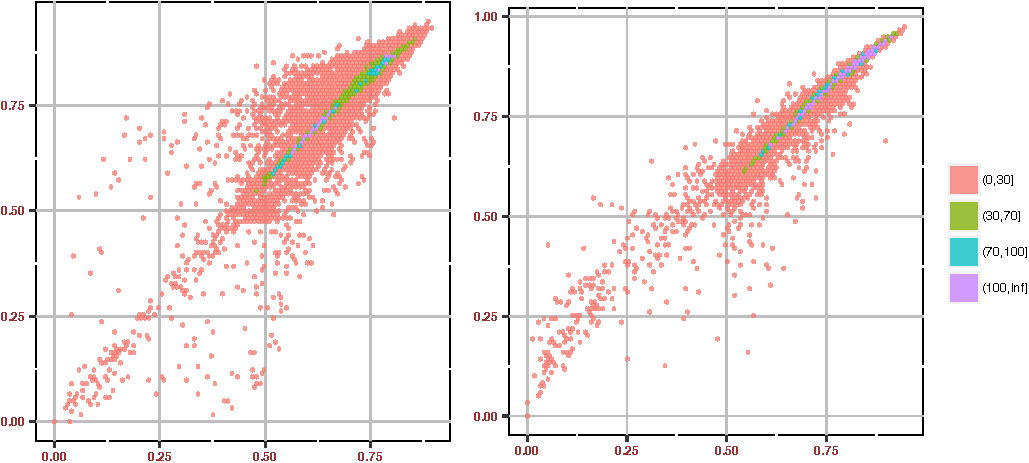
\includegraphics[width = 0.6\textwidth]{Figs/sim.pdf}
 \caption{ comparison of posterior probabilities of being DD among different number of subtypes, when we underestimate the number of subtypes, the difference is huge, see PDD between 6 subtypes and 7 subtypes. There is an approximate horizontal line with massive points at the top of left panel, which indicate that we underestimate lots of DD genes due to underestimate the number of subtypes. While in the case when we overestimate the number of subtypes 7 subtypes vs. 8 subtypes, though inflating PDD but the variation of difference is small, from 6 to 8 subtypes the PDD become more linear related.}
  \label{fig:6}
\end{figure}




\begin{comment}
\begin{figure}[h]
\vspace{-\parskip}
\minipage{0.5\textwidth}
  \includegraphics[width=\textwidth]{Figs/sim_67.png}
\endminipage\hfill
\minipage{0.5\textwidth}
  \includegraphics[width=\textwidth]{Figs/sim_78.png}
  \endminipage
\caption{comparison of posterior probabilities of being DD among different number of subtypes, when we underestimate the number of subtypes, the difference is huge, see PDD between 6 subtypes and 7 subtypes. There is an approximate horizontal line with massive points at the top of left panel, which indicate that we underestimate lots of DD genes due to underestimate the number of subtypes. While in the case when we overestimate the number of subtypes 7 subtypes vs. 8 subtypes, though inflating PDD but the variation of difference is small, from 6 to 8 subtypes the PDD become more linear related.}
\end{figure}
\begin{figure}[H]
  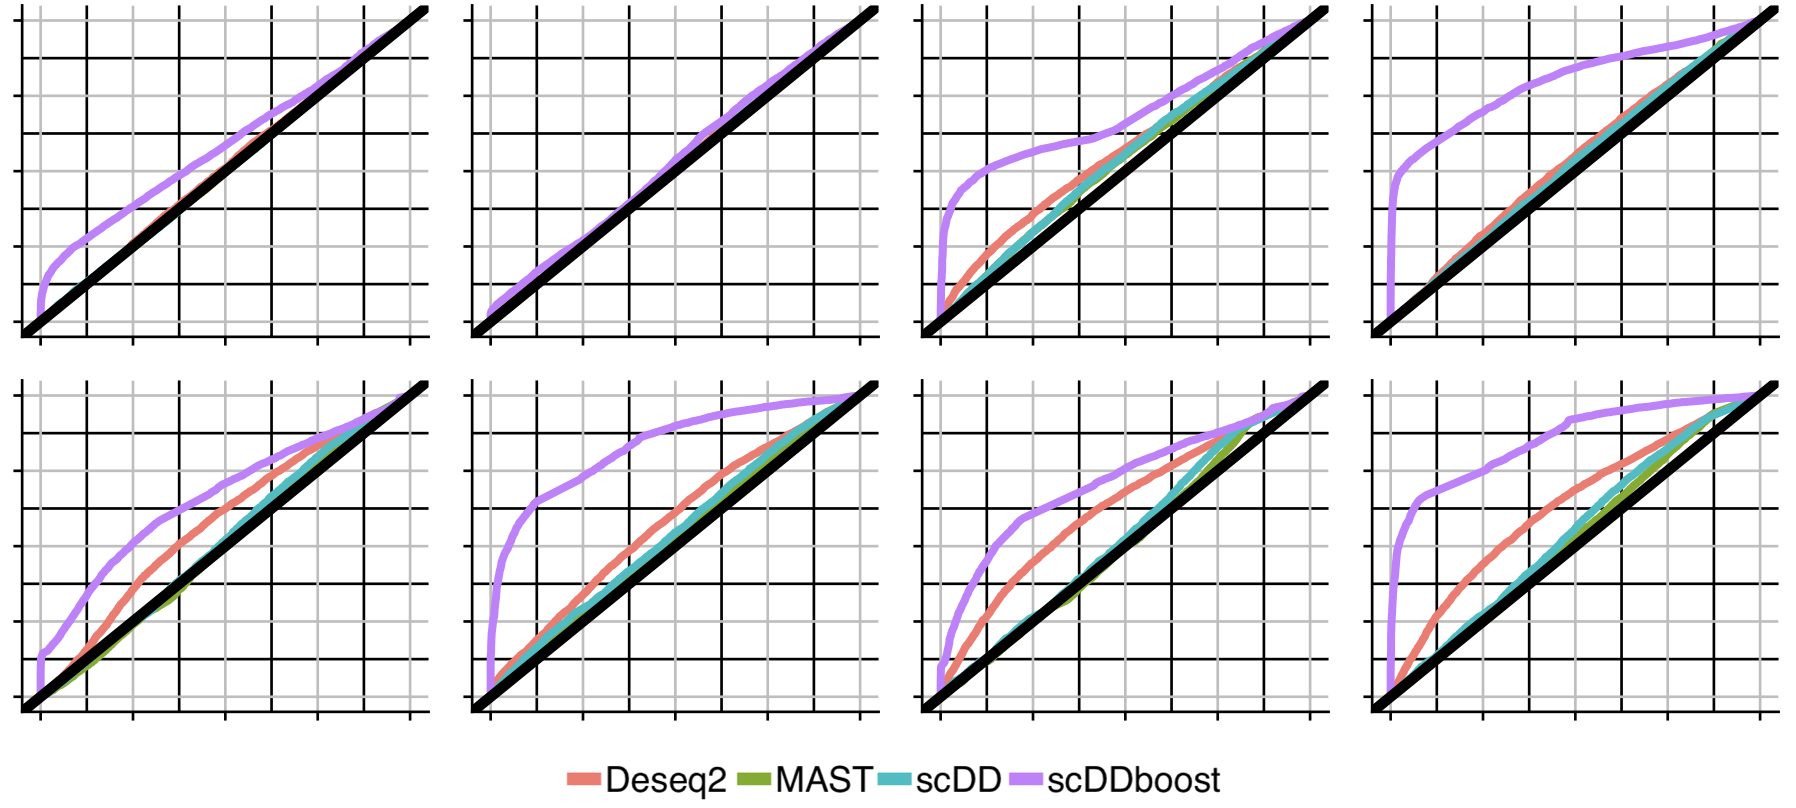
\includegraphics[width = 0.8\textwidth]{Figs/roc.png}
  \caption{Roc curve of scDDboost, scDD, MAST and DESeq2, scDDboost has largest area under the roc curve. Roc curves of other three methods are similar. For those roc curve there is bigger difference at low level of false positive rate, as scDDboost identified twice many true DD genes as other methods.  Roc curves are obtained under different settings of hyper parameters of simulations.}
  \label{fig:5}
\end{figure}
\end{comment}


Since we are modeling gene transcript within each subtype as negative-binomially distributed and we only test one parameter(mean) change among subtypes. In some scenario, it could be insufficient to model the variability within subtype. Even though there is no mean expression change among subtypes but more subtle distributional change occurred among subtypes changed, EBSeq would fail to detect the discrepancies between subtypes, thus limit power of scDDboost.\\


\subsection{Empirical study}


We use 13 datasets from conquer\cite{ref:Cq} to test performance of our method on empirical data. We compare our results with scDD\cite{ref:scDD}, MAST\cite{ref:MAST} and DESeq2\cite{ref:Des}, we have also investigated performance of scDDboost under different clustering method, (sc3\cite{sc3}, supplimentary)  and obtain similar \\
**see Supplementary Material Table S1**

\begin{figure}[H]
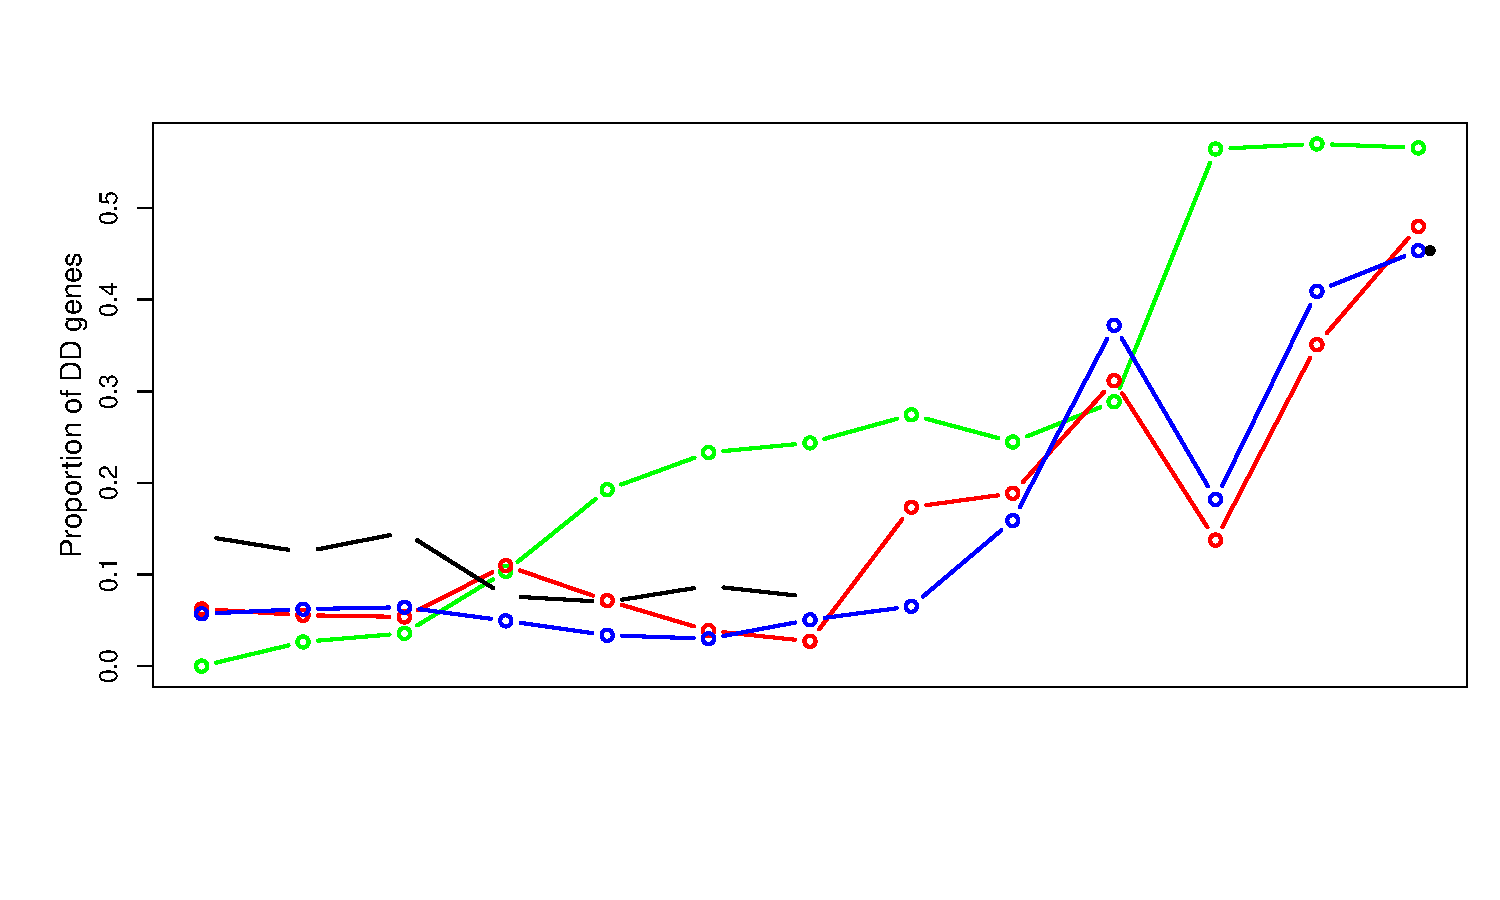
\includegraphics[width = 1\textwidth]{Figs/DD95.pdf}
 \caption{ number of DD genes with respect to total number of genes identified by each method. Ranked by mean list size}
  \label{fig:6}
\end{figure}



We found that bulk method DESeq2 tends to have the most number of DE genes. But among single cell methods, scDDboost usually identified the most DD genes. Further we observed quite a few genes uniquely identified by scDDboost are likely to have different distribution across conditions. For example, Fig 5, we use violin plot to demonstrate the log expression profiles among DEC and EC. \\
\begin{figure}[H]
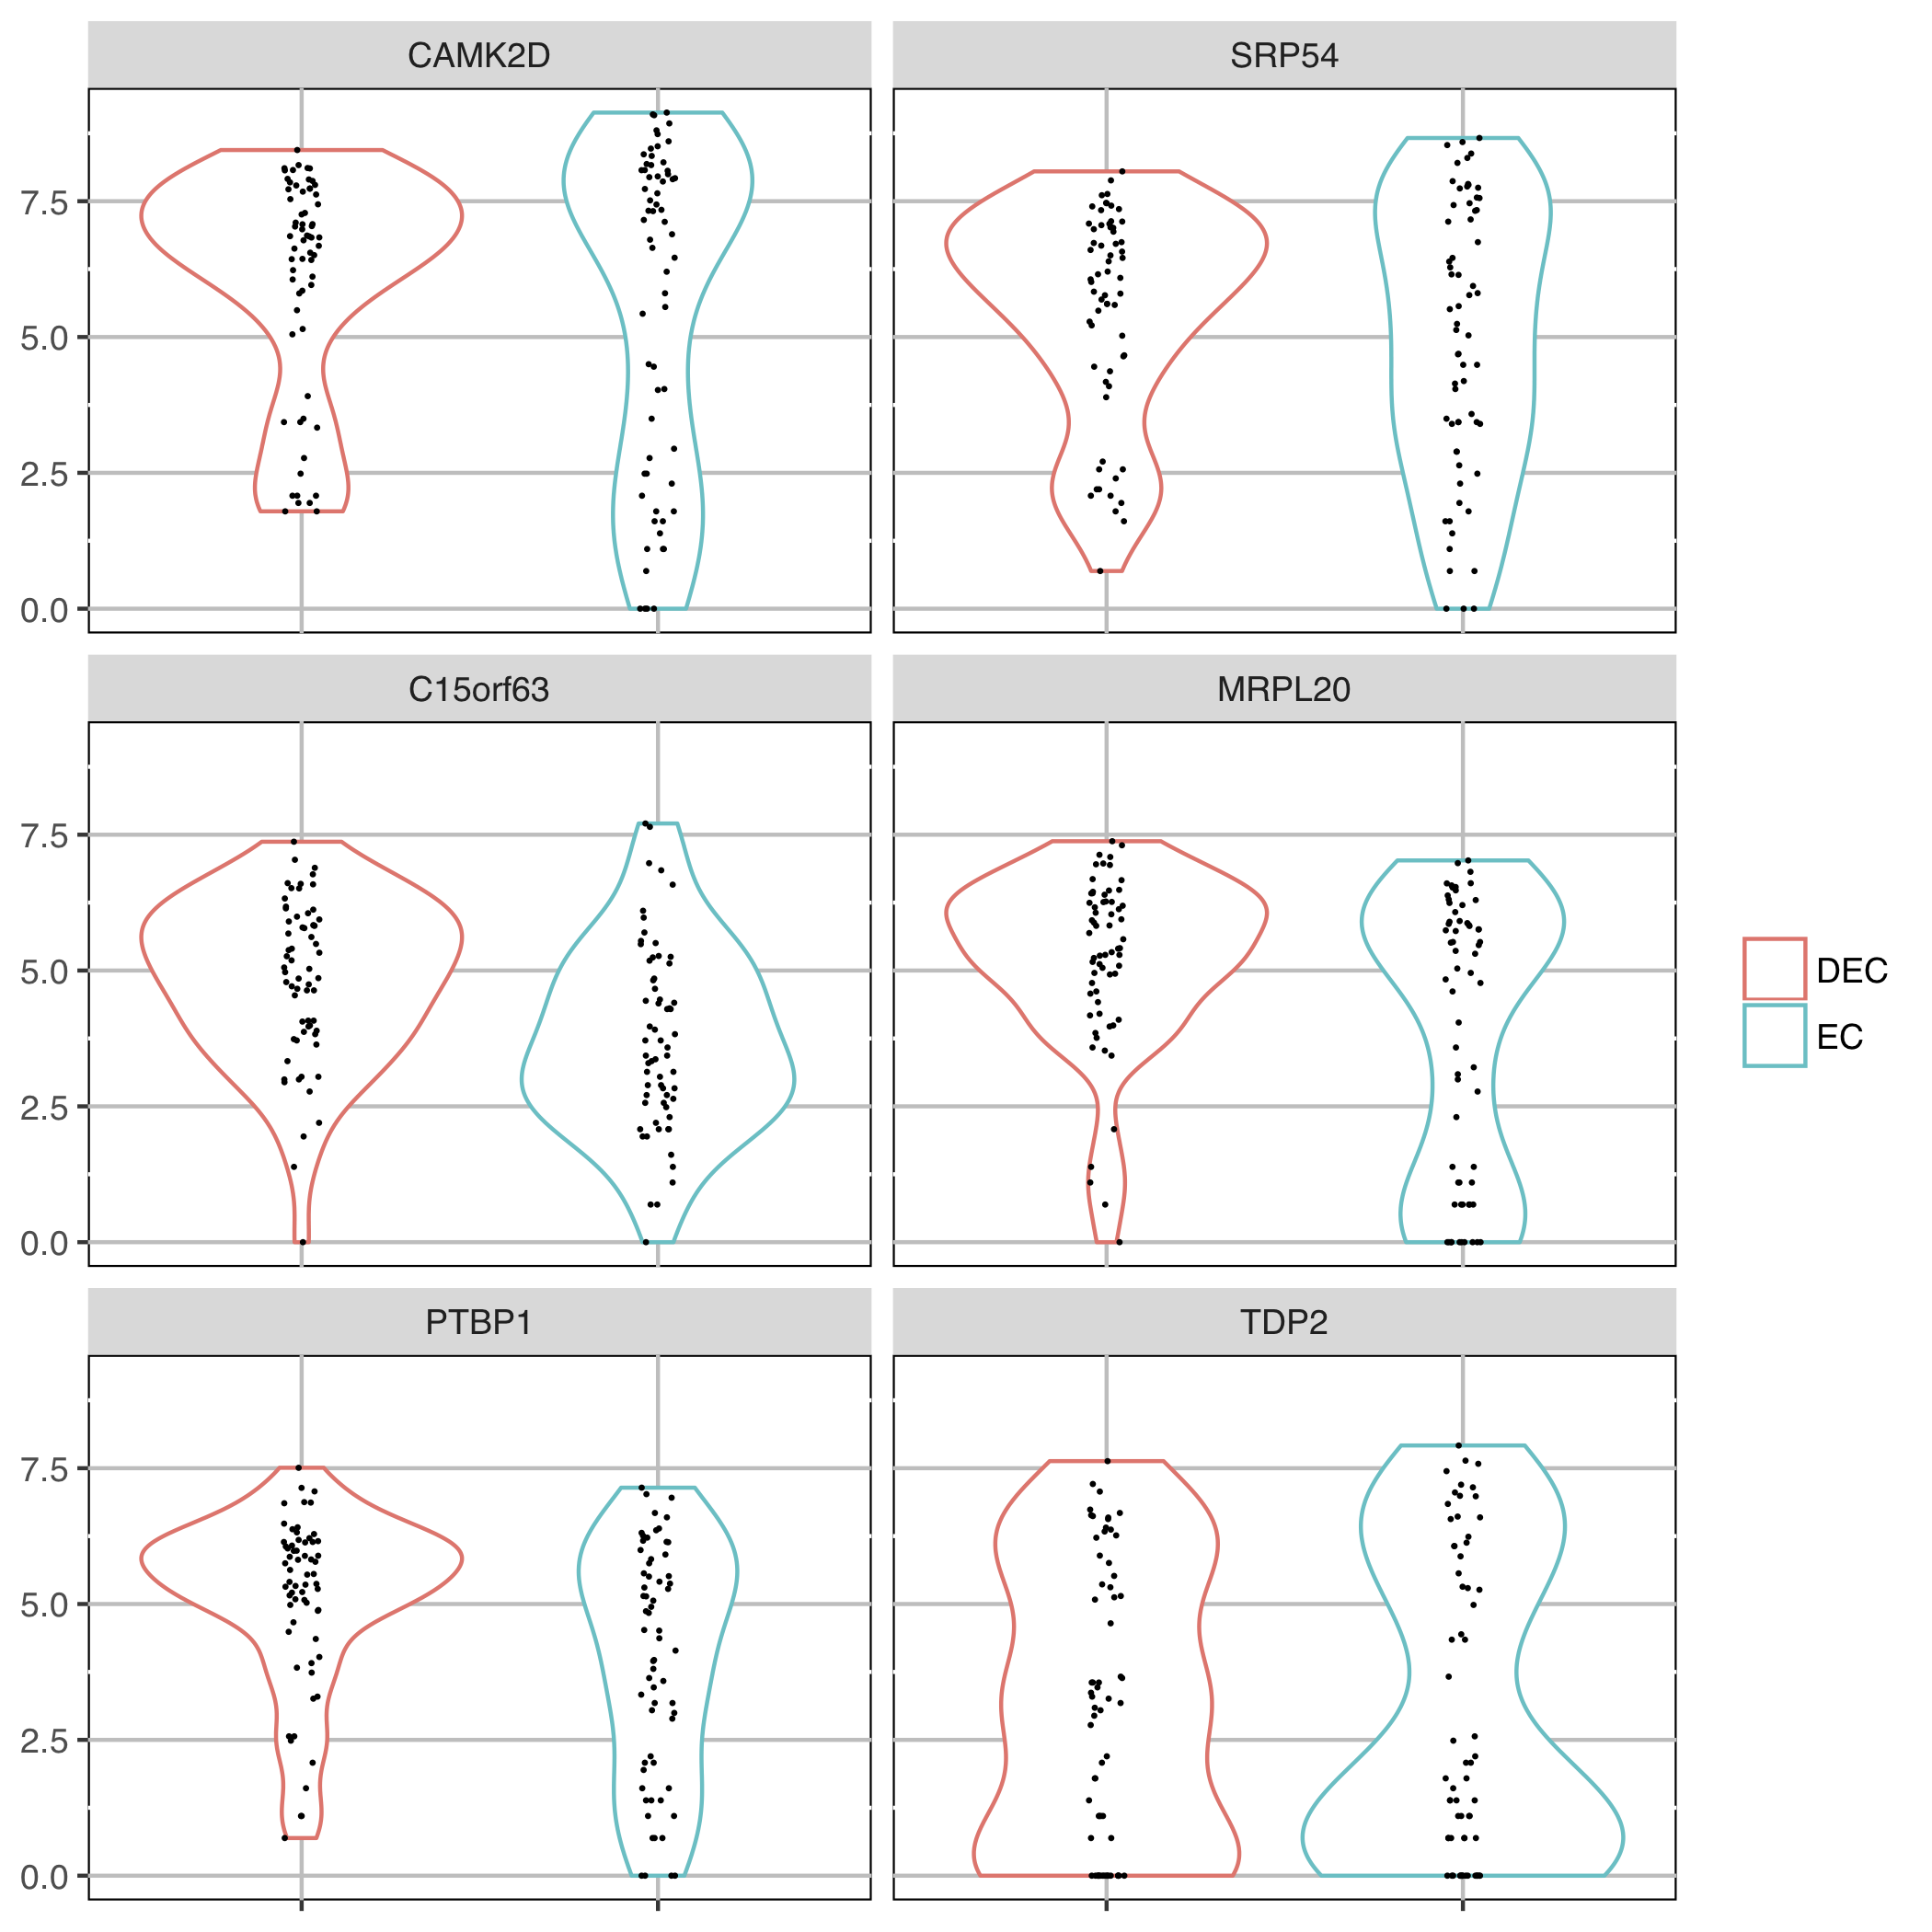
\includegraphics[width = 0.6\textwidth]{Figs/density_DEC_dd.png}
 \caption{ Densities of log transformed transcripts, 6 DD genes uniquely identified by scDDboost, for data GSE75748, DEC vs. EC, We observe some of the genes are different distributed across conditions.}
  \label{fig:6}
\end{figure}

\subsection{Empirical study: null cases}
Although bulk methods seems to be the most powerful one, we found it also has a higher false discovery rate comparing to single cell methods. We validate false discovery rate on ten null datasets from table 1. For each null dataset, we randomly split the cells from one condition into two subsets and test difference of gene expression between those subsets. Since the two subsets of cells actually came from same condition, there should not be any differential distributed genes, any positive call would be a false positive. We repeat the random split and testing for five times on each null data set. We evaluate the type I error control for the methods returning nominal p-values, by recording the fraction of genes(with a valid p-value) that are assigned a nomial p-value below 0.05 (Fig 6).\\
scDDboost could control FDR since we assume cells are sampled from population composed of different subtypes. Cells from one subtype are equal likely to be assigned to either one of the two subsets. Consequently, it is very likely that proportions of subtypes remain unchanged among the two subsets.

\begin{table}[ht]
\small
\centering
\begin{tabular}{ |p{3cm}|p{5cm}|p{3cm}|p{2cm}|}
\hline
 Data set & Conditions & Number of cells/condition & Organism \\
\hline
\hline
GSE57872null & patient1 & 96,96 & human \\
\hline
GSE52529null & T0 & 48, 48 & human \\
\hline
GSE48968-GPL13112null & BMDC (2h LPS stimulation) & 48,48 & mouse \\
\hline
 GSE60749-GPL13112null & v6.5 mouse embryonic stem cells, culture conditions: 2i+LIF & 45,45 & mouse \\
 \hline
 GSE74596null & NKT1 & 23,23 & mouse\\
 \hline
 EMTAB2805null & G1 & 48,48 & mouse\\
 \hline
GSE71585-GPL13112null &Gad2tdTpositive  & 40,40 & mouse \\
\hline
GSE64016null & G1 & 46,45 & human \\
\hline
GSE79102null & patient1 & 26, 25 & human\\
\hline
\end{tabular}
\captionof{table}{datasets used for null cases, as cells are coming from same biological condition, there should not be any differential distributed genes, any positive call is false positive}
\end{table}


\begin{figure}[H]
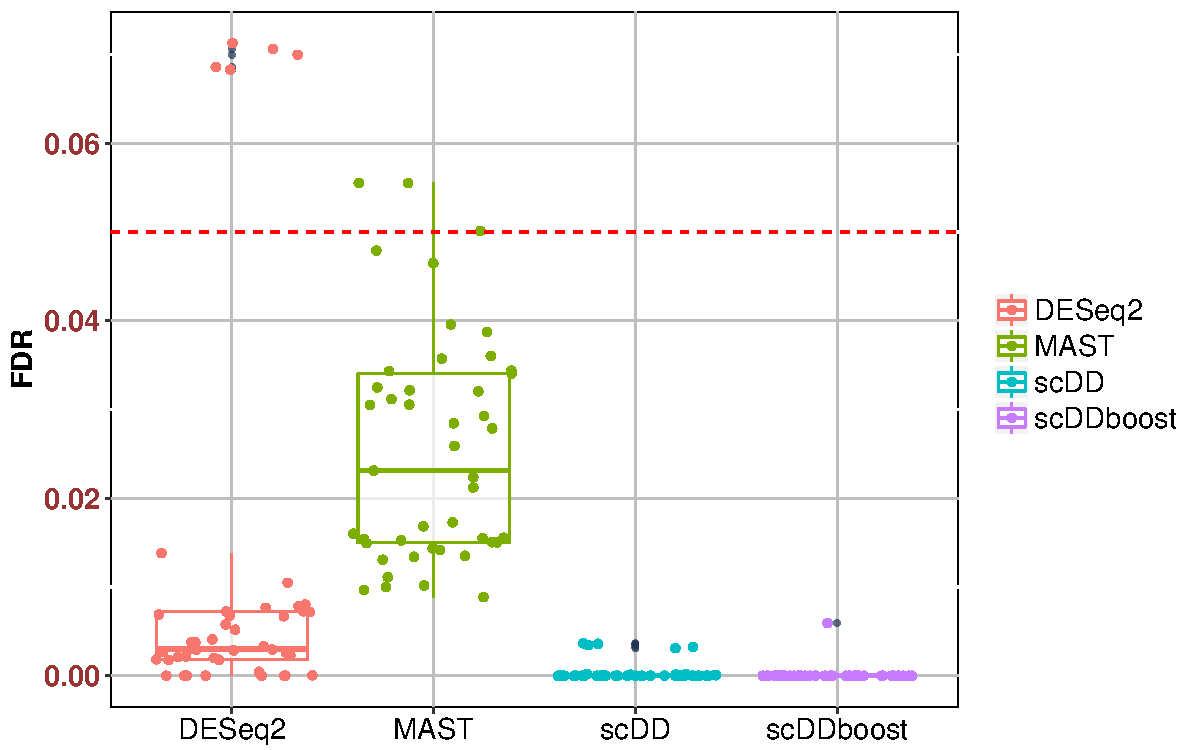
\includegraphics[width = 0.7\textwidth]{Figs/fdr.pdf}
 \caption{FDR of scDDboost, scDD, MAST and DESeq2 on null dataset from table 1, DESeq2 usually identify a lot but may lose the control of type I error. While other single cell methods could control FDR. }
  \label{fig:7}
\end{figure}

\subsection{Number of subtypes}
***label for graph, update later***

From our empirical experience, it is typical $K$ will not be larger than 8. We demonstrate the change of posterior probabilities of differential distribution given different number of subtypes at data GSE75748 and GSE48968. In both cases, if allowing one more subtype would result in a lot increases in posterior probabilities, which suggests that the number of subtypes is underestimated since we found more distribution differences between conditions given one more mixture component. If posterior inference is stable after increasing the number of subtypes, then we consider previous number of subtypes to be optimal. 
\begin{figure}[H]

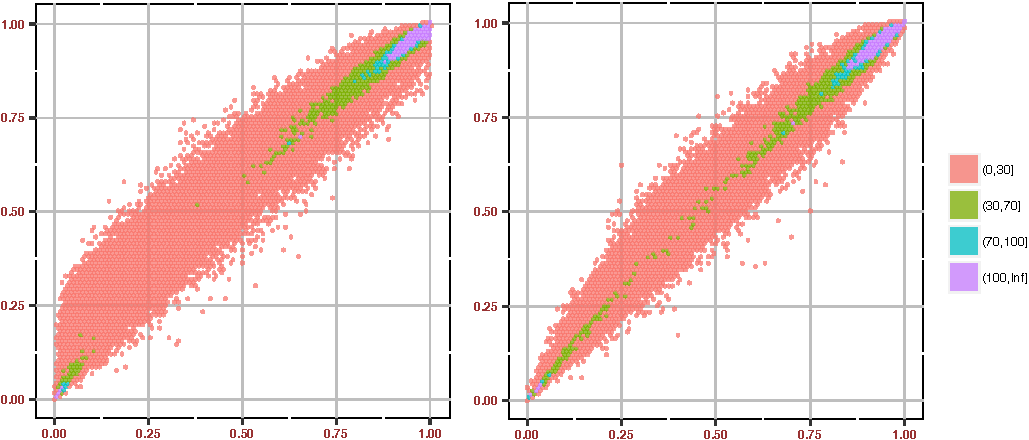
\includegraphics[width = 0.7\textwidth]{Figs/s_78_GSE57872.pdf}

\begin{comment}

\minipage{0.5\textwidth}
  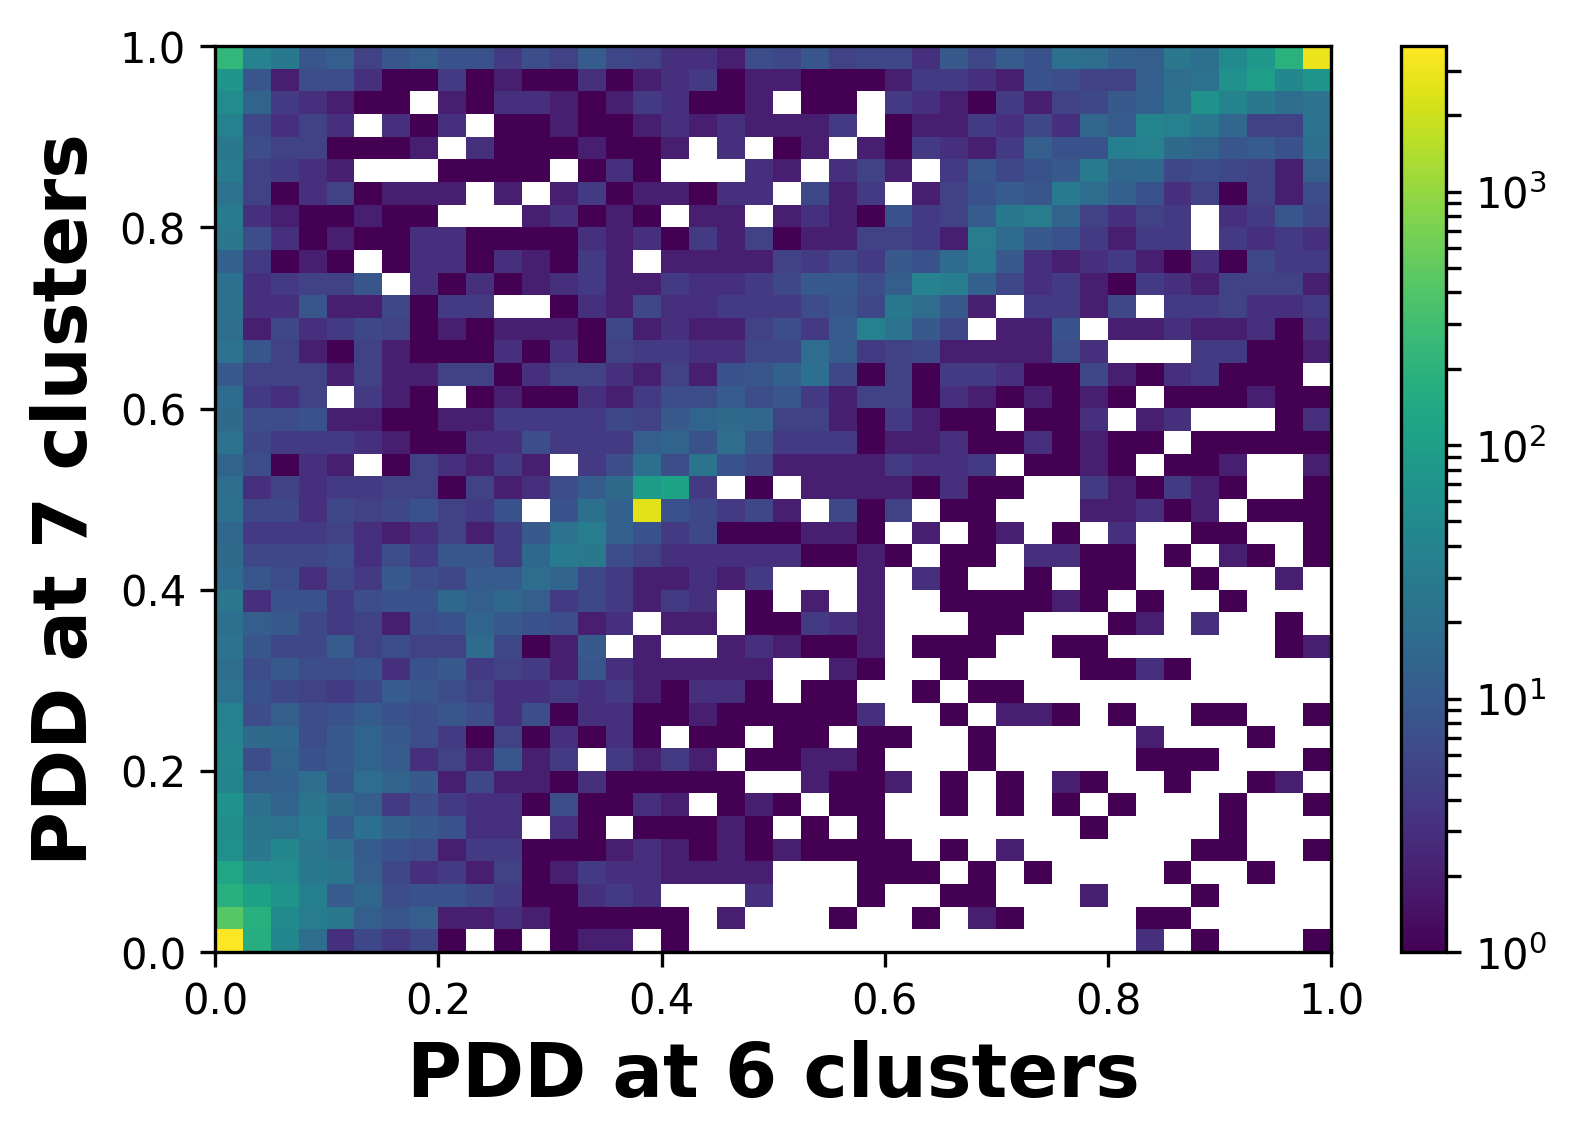
\includegraphics[height = 5cm, width=\linewidth]{Figs/DN_67.png}
\endminipage\hfill
\minipage{0.5\textwidth}
  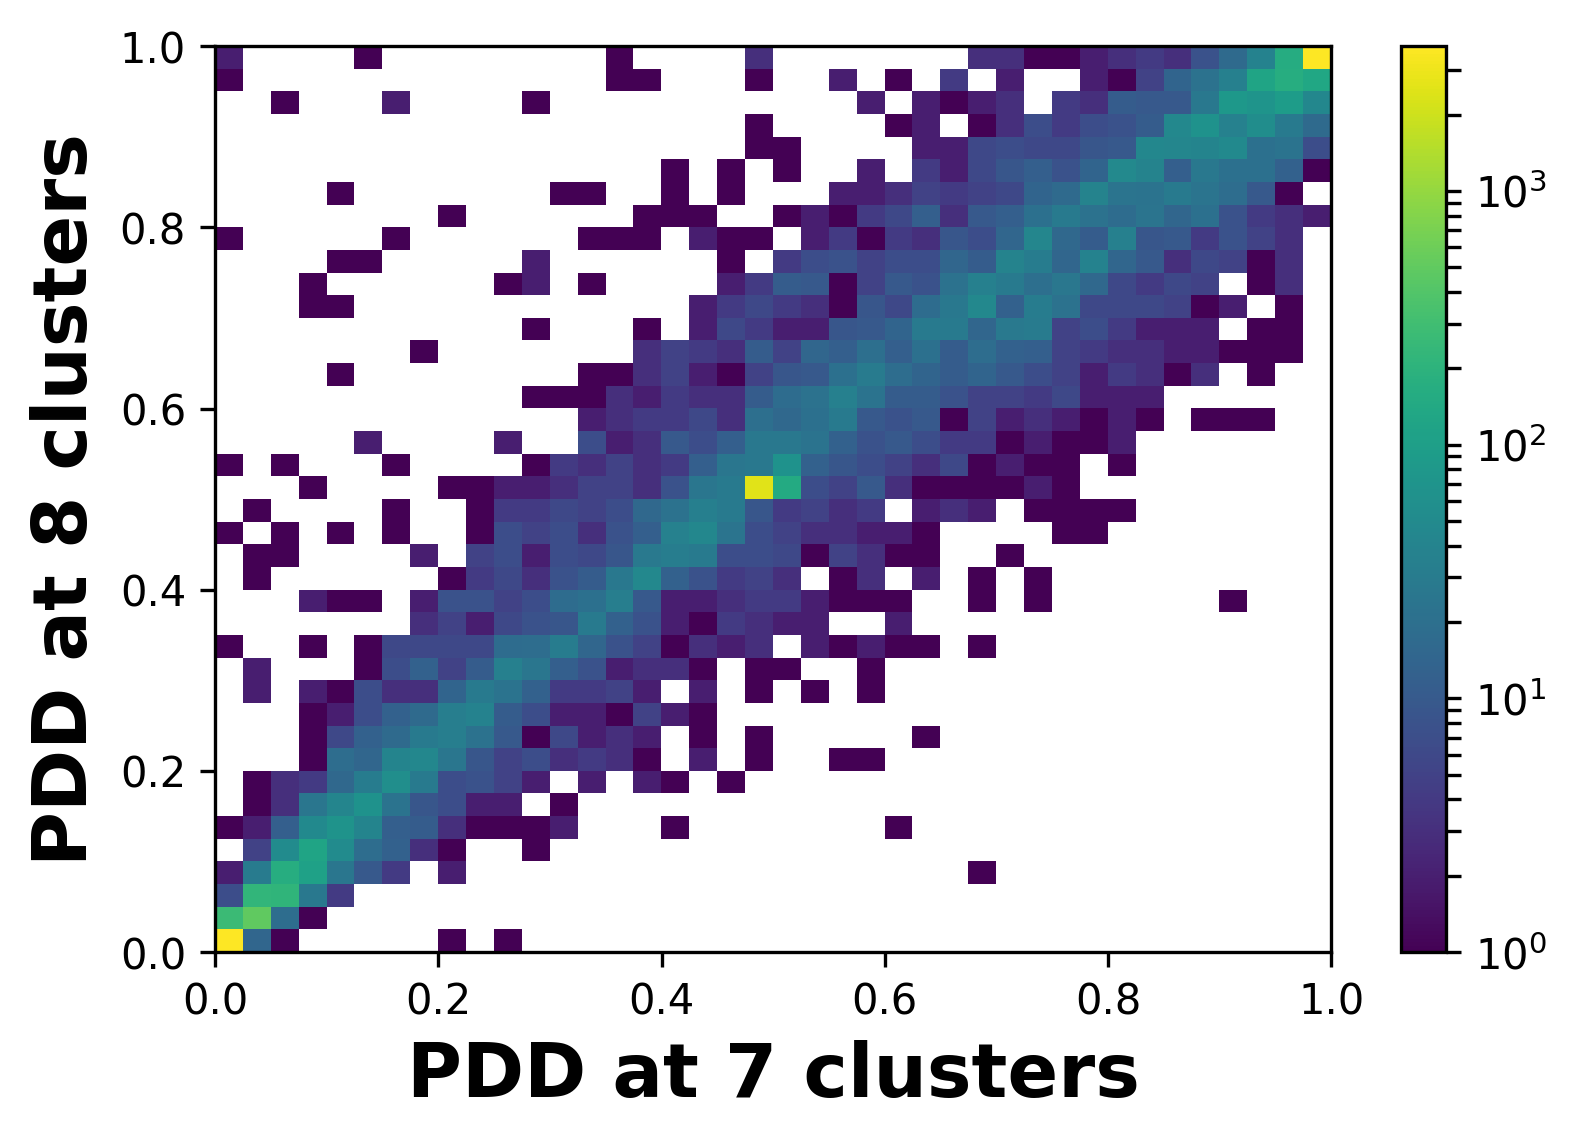
\includegraphics[height = 5cm, width=\linewidth]{Figs/DN_78.png}
\endminipage\hfill

\end{comment}

\caption{selecting number of subtypes for data GSE57872, we observe posterior probabilities become stable at more than 6 subtypes. Since increasing number of subtypes tends to decrease sample size of each subtypes, make complicate constraints for equivalent distribution and inflate estimated PDD.  We select number of subtypes to be 7}
\end{figure}


\begin{figure}[H]

\begin{comment}

\minipage{0.5\textwidth}
  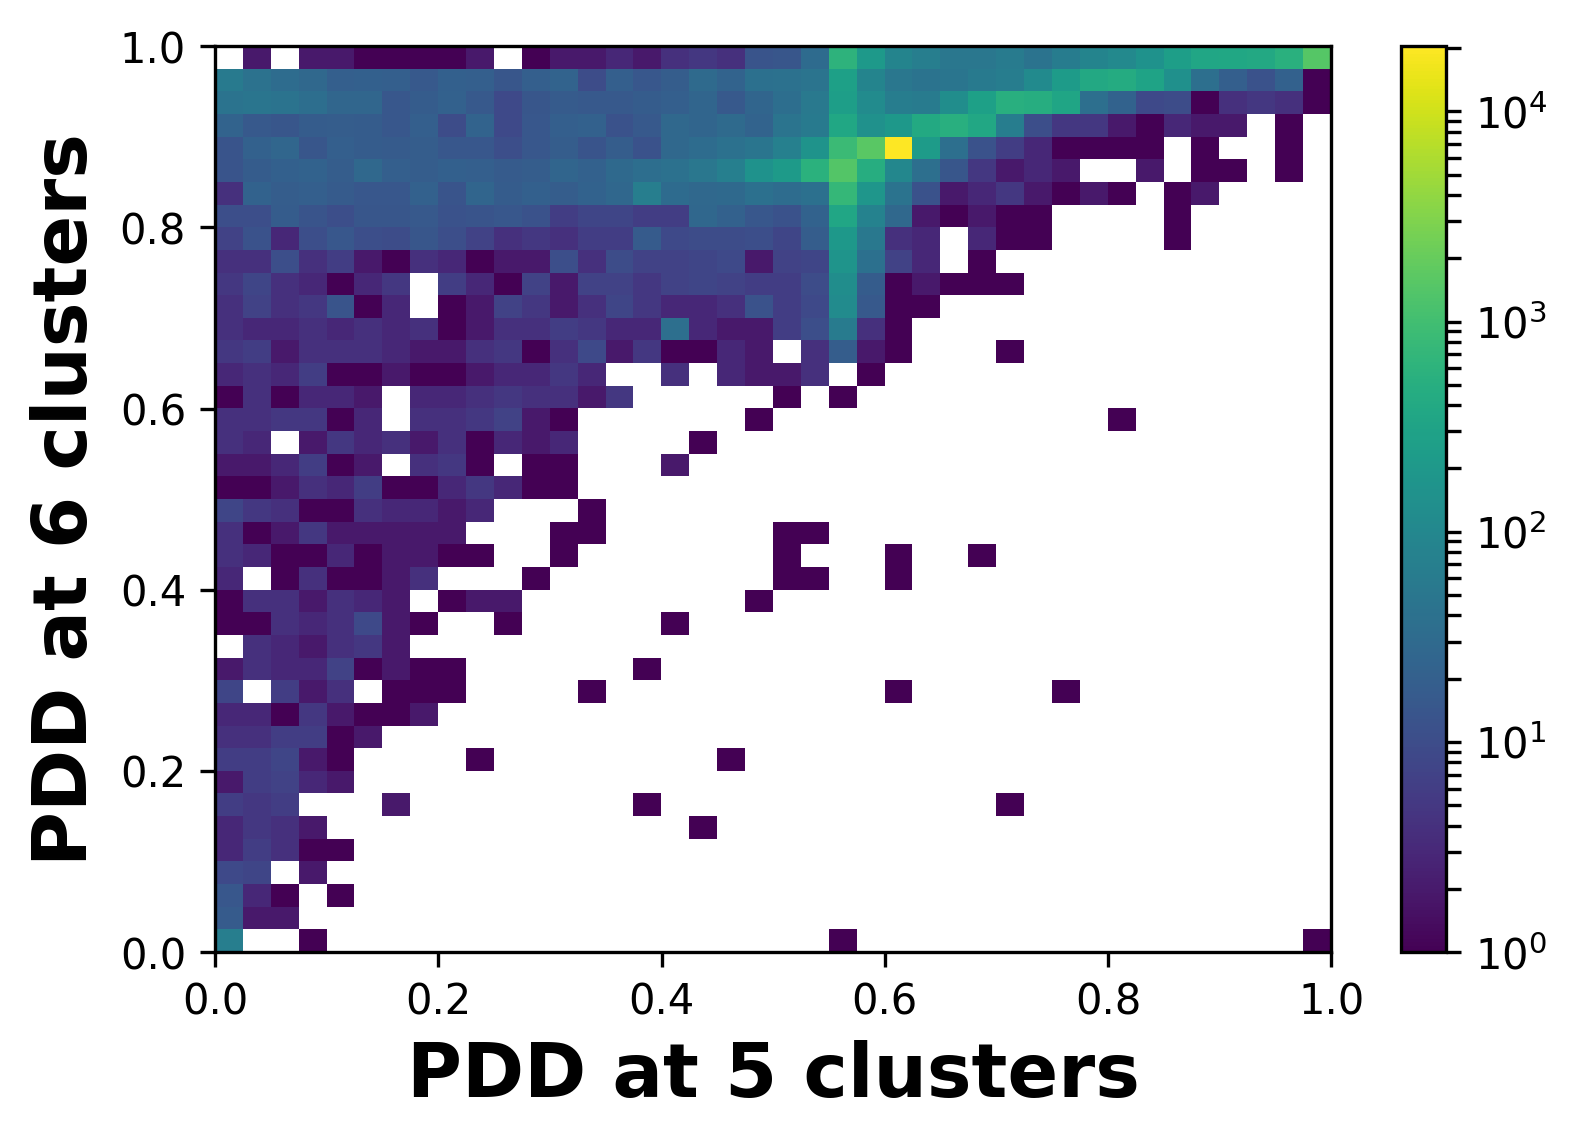
\includegraphics[height = 5cm, width=\linewidth]{Figs/G48_56.png}
\endminipage\hfill
\minipage{0.5\textwidth}
  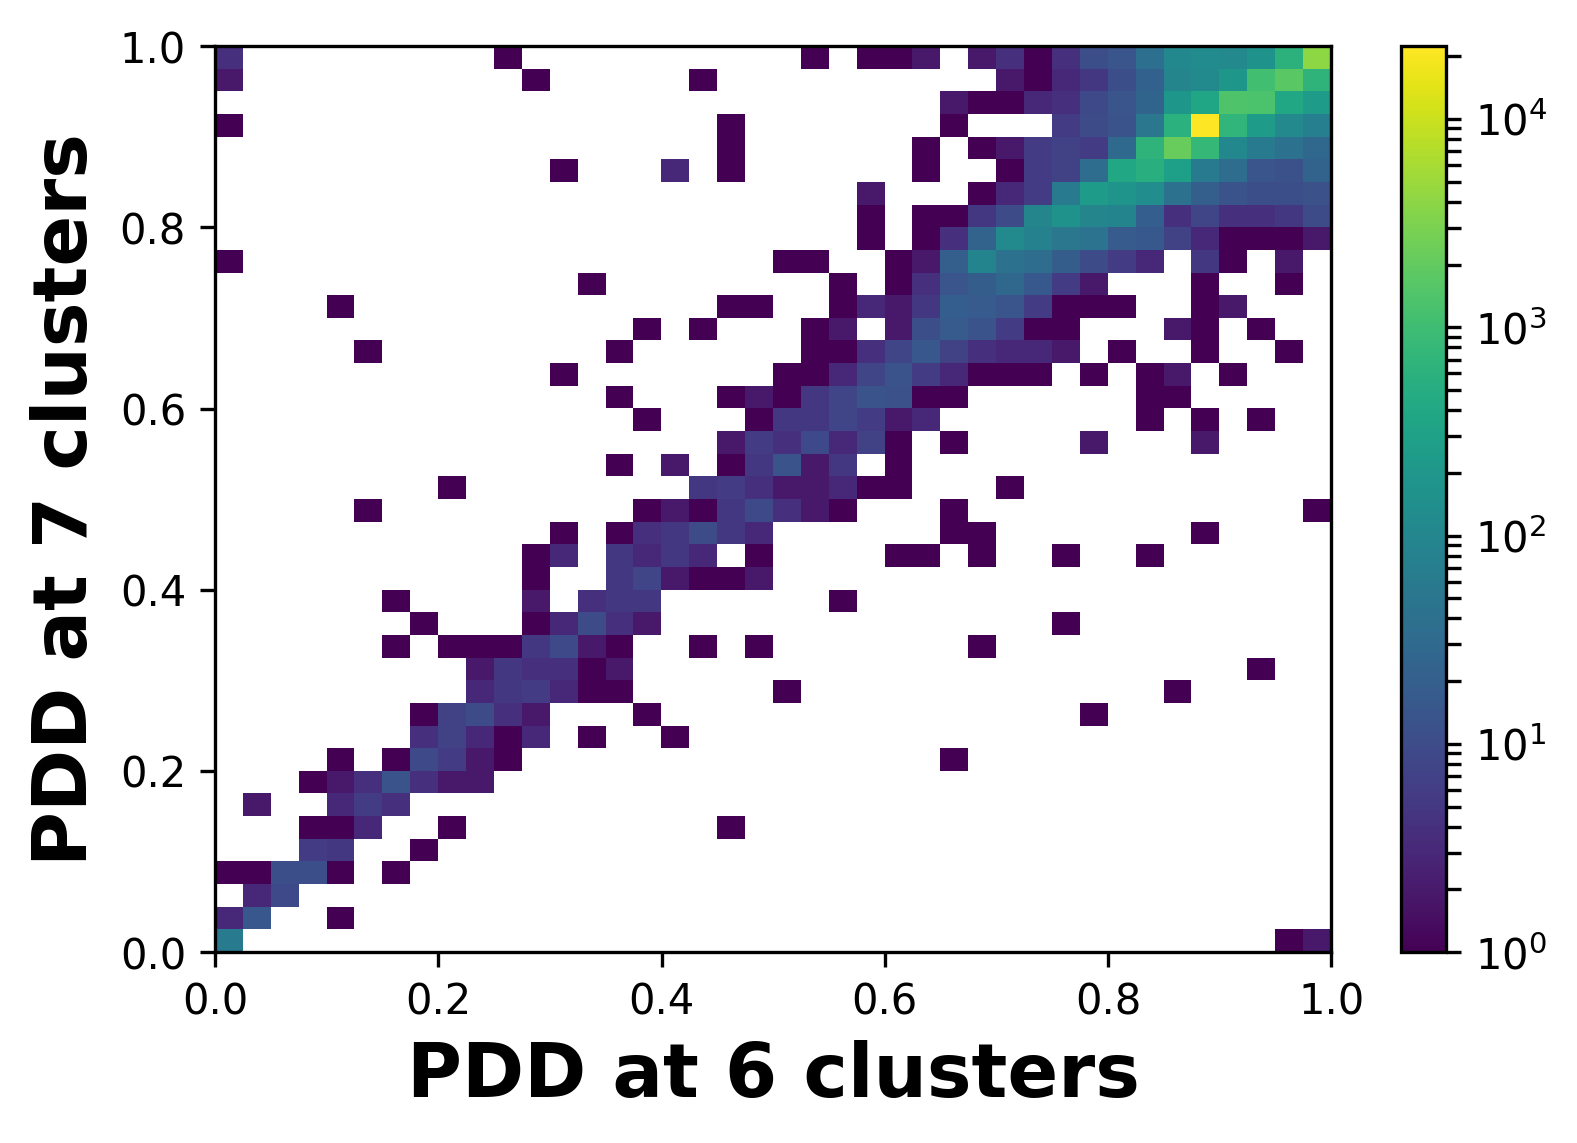
\includegraphics[height = 5cm, width=\linewidth]{Figs/G48_67.png}
\endminipage\hfill
\end{comment}

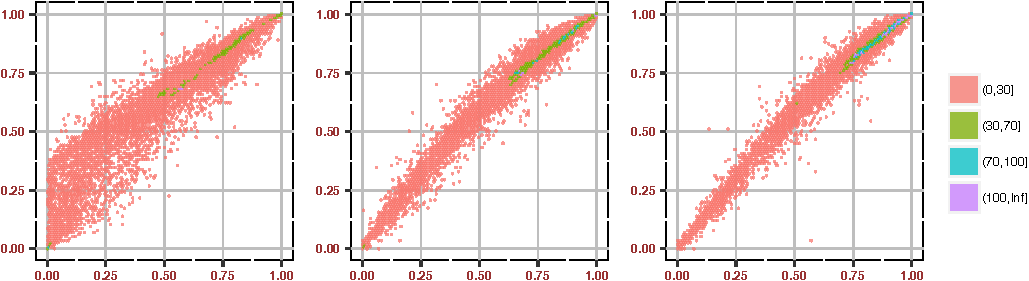
\includegraphics[width = 1\textwidth]{Figs/s_789_GSE48968.pdf}

\caption{selecting number of subtypes for data GSE48968, we observe posterior probabilities become stable at more than 5 subtypes}
\end{figure}


\subsection{Bursting parameters}

***on the method estimated p-value, update later***

D3E\cite{ref:d3e} is a distributional method that can identify bursting parameters of transcripts. Rate of promoter activation, rate of promoter inactivation and the rate of transcription when the promoter is in the active state are estimated by D3E.  We investigate DD genes identified by scDDboost and their change of those three parameters on dataset EMTAB2805\\

\begin{figure}[H]

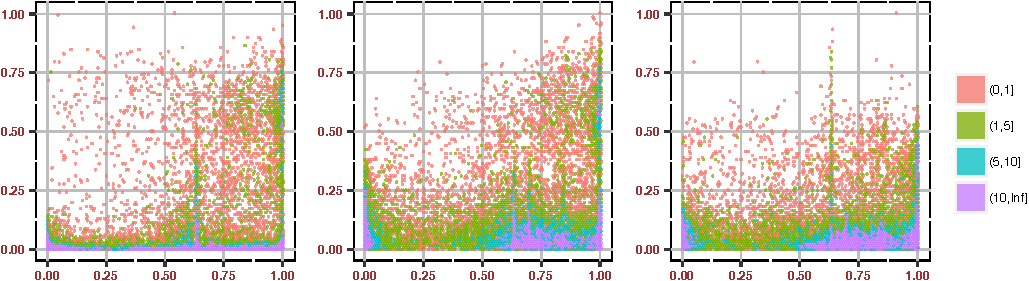
\includegraphics[width = 1\textwidth]{Figs/d3eplot.pdf}

\caption{D3E method will estimate 3 bursting parameters probability of a gene being on (\textbf{a}) and off (\textbf{b}) and the expression rate when the gene expression is on (\textbf{c}), we plot the hexbin plot of probability of a gene being DD under out method v.s. the absolute value of log fold change of \textbf{a} , \textbf{b} and \textbf{c}  across the two conditions accordingly. The log fold change is scaled by dividing the largest log fold change so that ends up in a value between 0 and 1 Here we use the GSE71585 data }
\end{figure}



\begin{comment}
\begin{figure}[H]
\vspace{-\parskip}
\minipage{0.33\textwidth}
  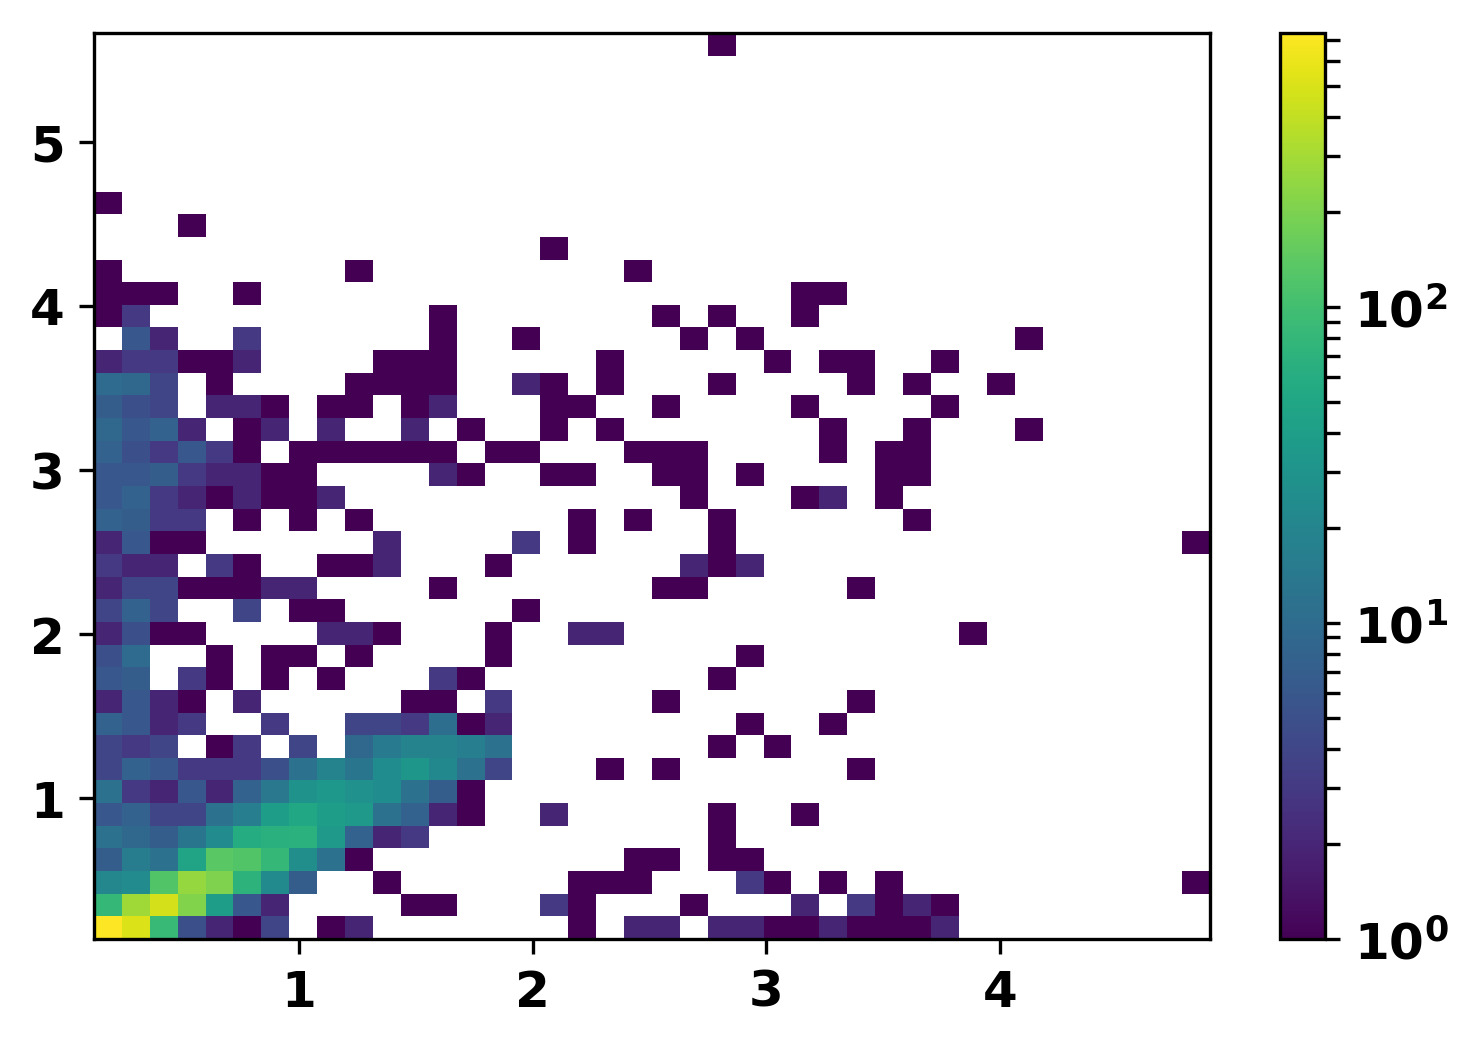
\includegraphics[clip,width=\textwidth]{Figs/act.png}
\endminipage
\minipage{0.33\textwidth}
  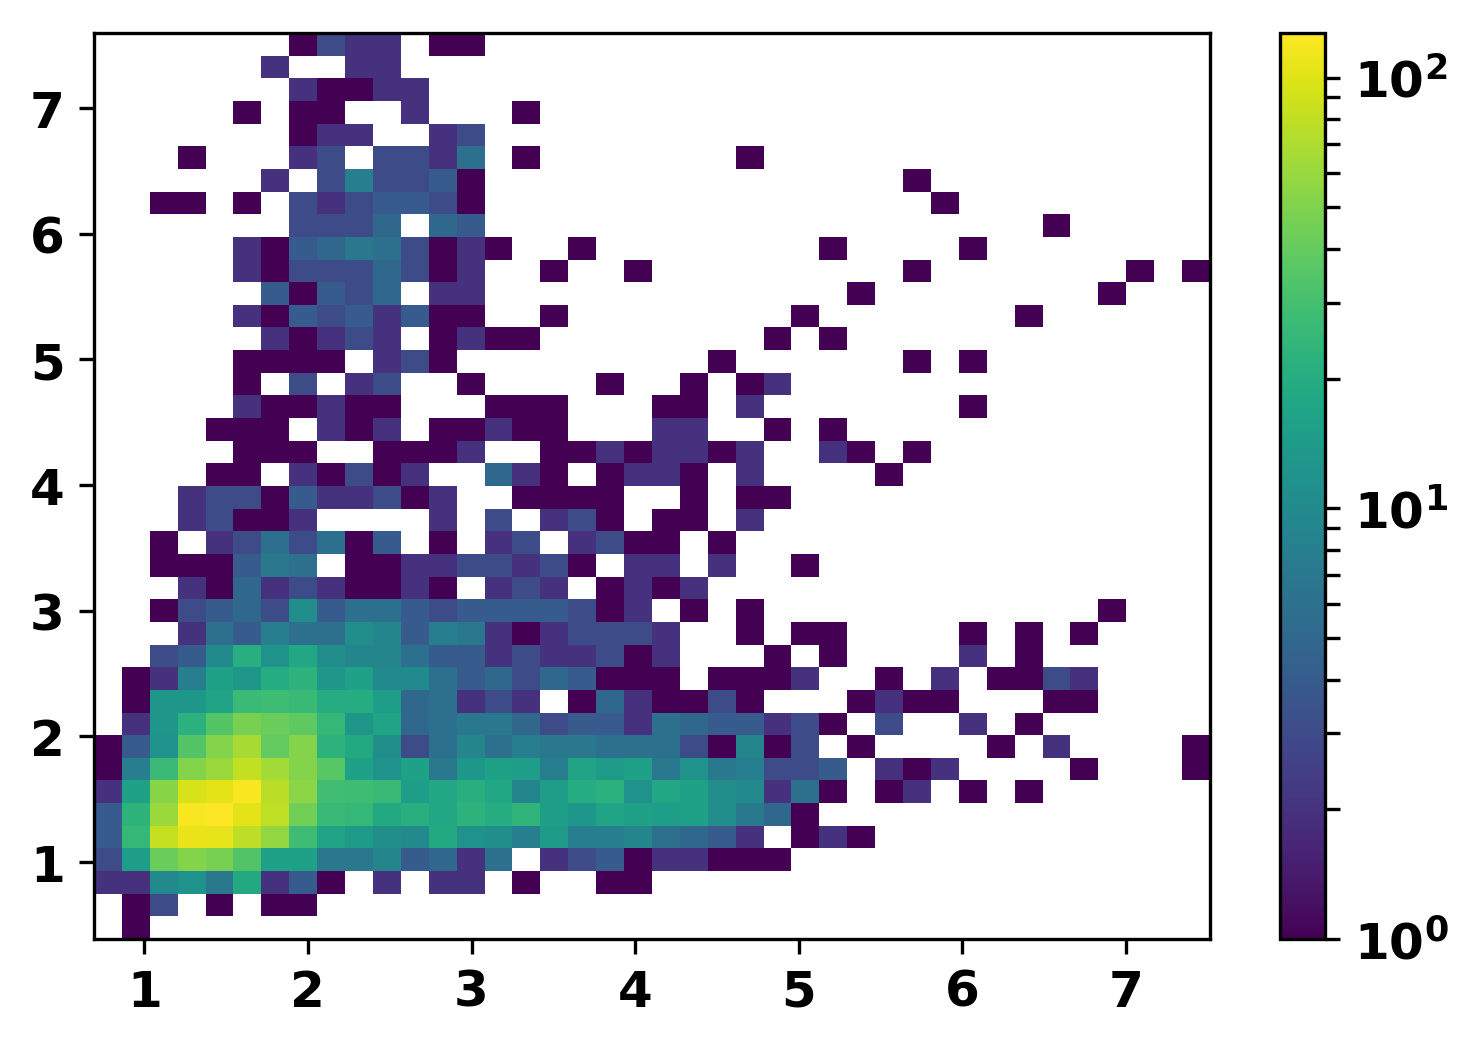
\includegraphics[clip,width=\textwidth]{Figs/in_act.png}
  \endminipage
 \minipage{0.33\textwidth}
  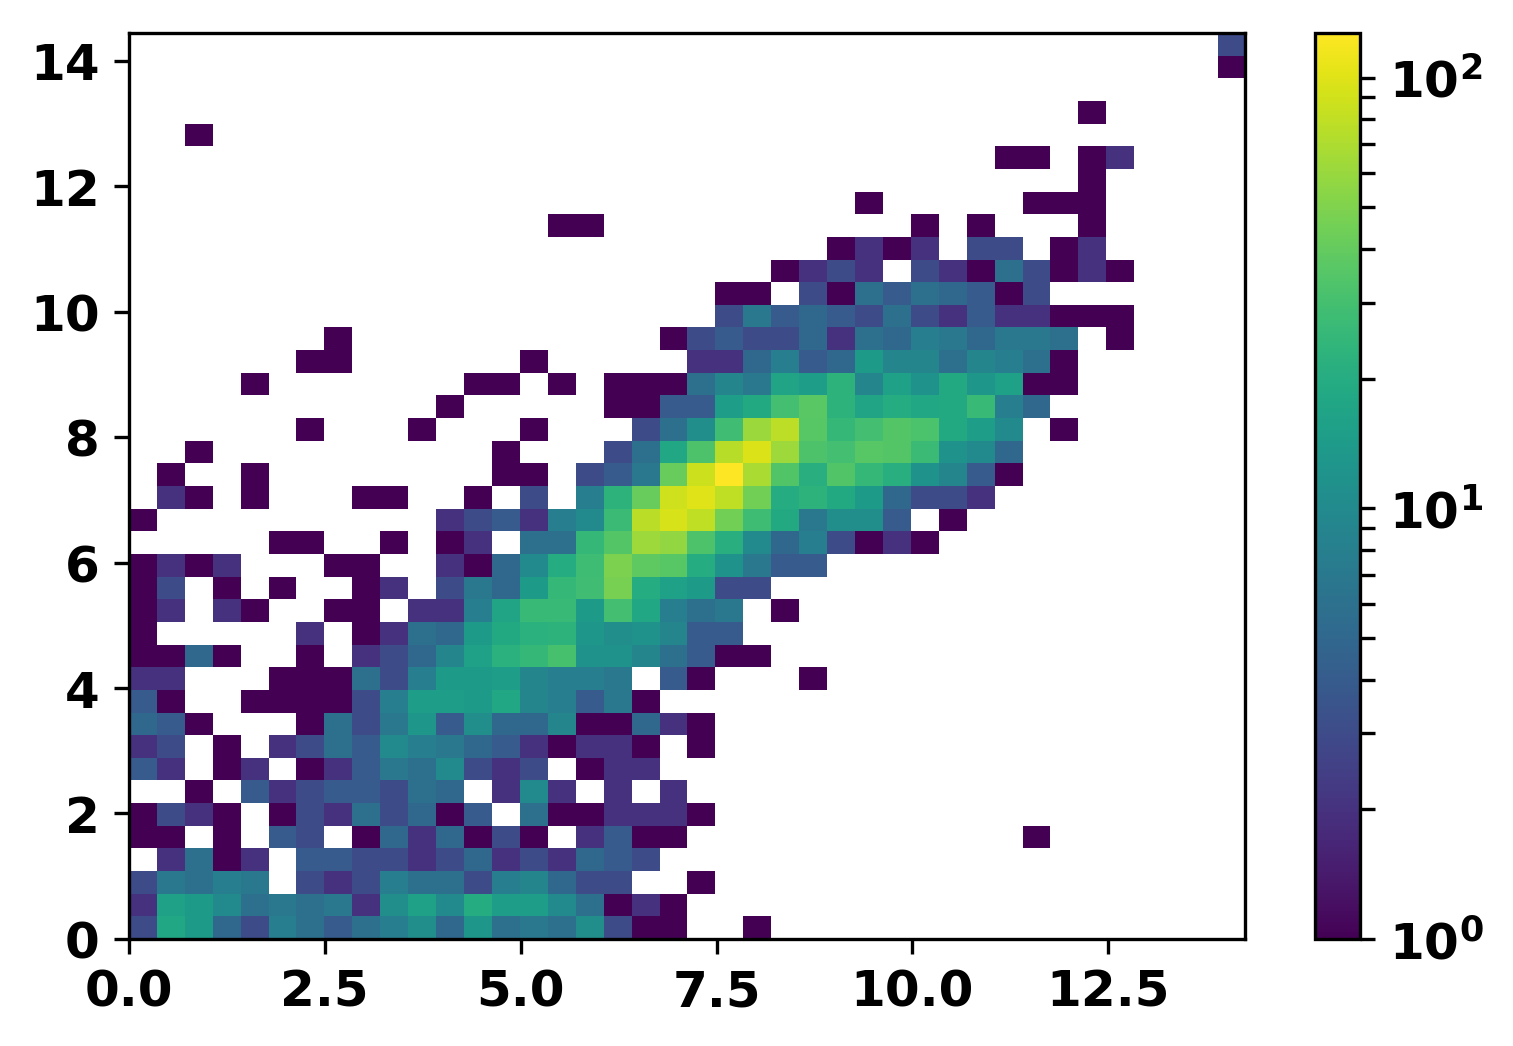
\includegraphics[clip,width=\textwidth]{Figs/t_rate.png}
  \endminipage
\captionof{figure}{2D histogram for bursting parameters of DD genes identified by scDDboost from dataset EMTAB2805 estimated by D3E. Left panel  : comparison of rate of promoter activation between two conditions, similarly, middle panel  : rate of promoter inactivation and right panel: rate of transcription when the promoter is in the active state. We observe that difference between transcription rate is smaller compare to difference between the activation and inactivation rate.}
\end{figure}
\end{comment}

We observed that DD genes identified by scDDboost tends to have similar transcription rate when the promoter is active across condition, while there are lots of variabilities in the action and inactivation rate. Estimations from D3E reveals that the major factor to drive DD genes are activation and inactivation rate (proportions of different subtyps), it make sense to consider mixture model like scDDboost.



\section{Theoretical issues}
\subsection{Posterior consistency}
Under some parameters settings, the double dirichlet prior will have limited resolution and lead to inconsistency of posterior probabilities, which we investigate with the following asymptotic analysis.

We first give the expression of posterior probability. Since there is no information favorable of any particular $A_\pi$, we select discrete uniform distribution as the prior for it, then the posterior probability is
\begin{align}
p(A_\pi | t^1, t^2) = c*\sum_{\pi' \text{ refines } \pi} p(t^1 | t^1_{\pi'})\, p(t^2 |  t^2_{\pi'} )
 \, p( t^1_{\pi'}, t^2_{\pi'} | A_{\pi'} )
\end{align}
for a normalizing constant $\frac{1}{c} = \underset{\pi' \in \Pi}\sum p(t^1 | t^1_{\pi'})\, p(t^2|  t^2_{\pi'} )
 \, p( t^1_{\pi'}, t^2_{\pi'} | A_{\pi'} )$.
 
Let $\Omega = \{(\phi, \psi): \overset{K}{\underset{i = 1}\sum}\phi_i = \overset{K}{\underset{i = 1}\sum}\psi_i = 1, \phi_i \geq 0, \psi_i \geq 0 , i = 1,..., K\}$ be the whole space. There is a subset of $\Omega$ we lack posterior inference. Let us first see an example:
\begin{figure}[h]
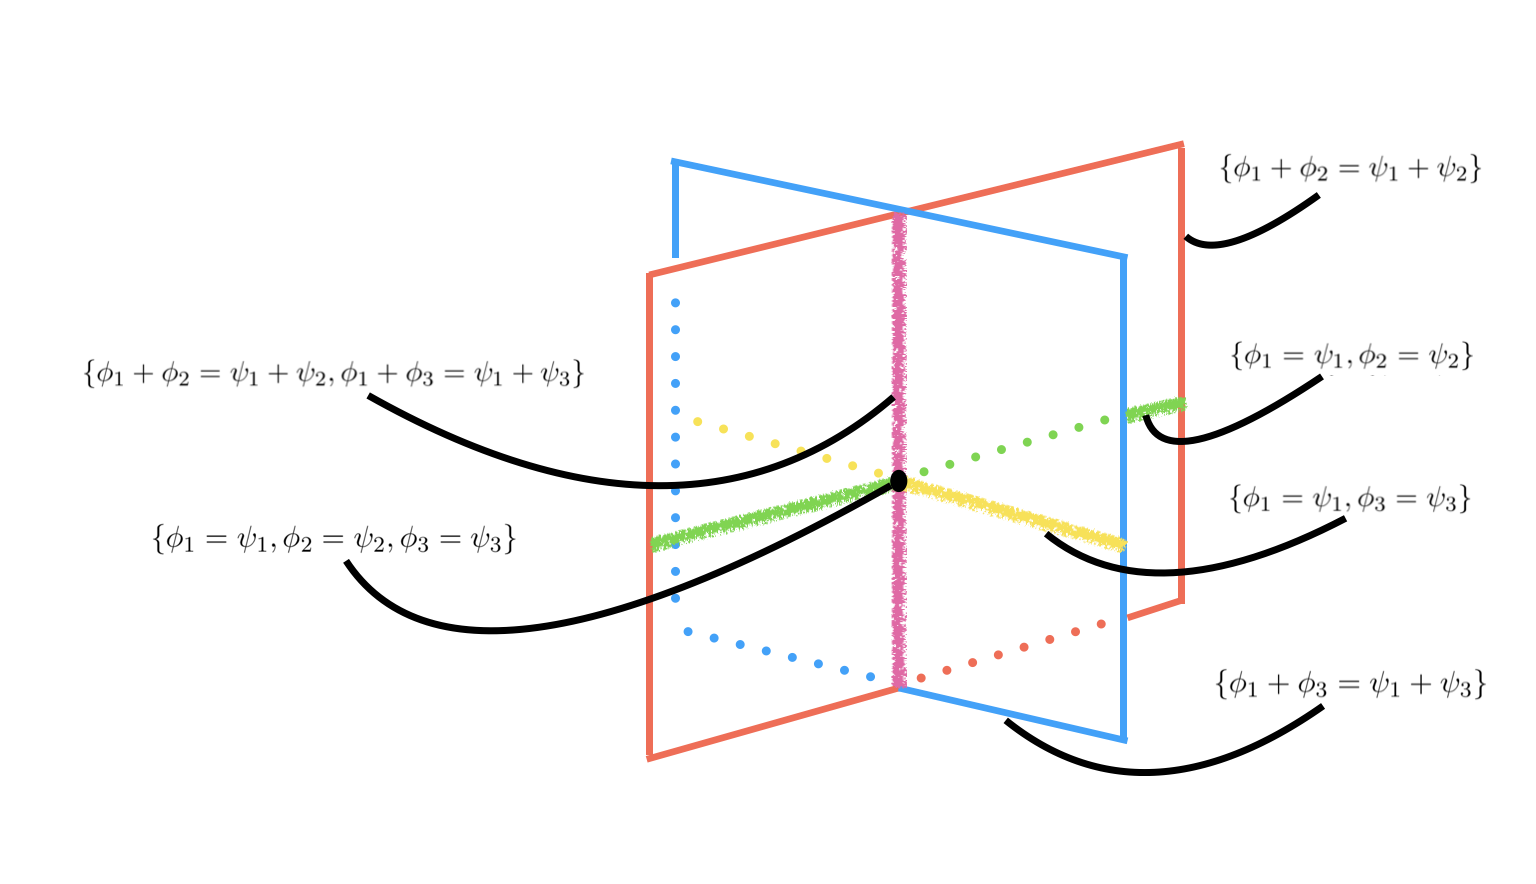
\includegraphics[scale = 0.5]{Figs/overlap.png}
 \caption{Four subtypes of cells,  simplexes of $(\phi,\psi)$ satisfying different constraints.}
  \label{fig:1}
\end{figure}
\hfill\\
In Fig 10, there are four subtypes, the rectangle with magenta boundary is a simplex $A_{\pi_1} = \{(\phi,\psi) : \phi_1 + \phi_2 = \psi_1 + \psi_2\}$, the rectangle with blue boundary is a simplex $A_{\pi_2} = \{(\phi,\psi) : \phi_1 + \phi_3 = \psi_1 + \psi_3\}$. The green line refers to $A_{\pi_3} = \{(\phi,\psi) : \phi_1 = \psi_1, \phi_2 = \psi_2\}$, the yellow line refers to $A_{\pi_4} = \{(\phi,\psi) : \phi_1 = \psi_1, \phi_3 = \psi_3\}$, the purple line refers to $A_{\pi_5} = \{(\phi,\psi) : \phi_1 + \phi_2 = \psi_1 + \psi_2, \phi_1 + \phi_3 = \psi_1 + \psi_3\}$, which is the intersection of $A_{\pi_1}$ and $A_{\pi_2}$, and finally the black dot which is the intersection of those three lines refers to the simplex with finest partitions, $\phi_i = \psi_i, \forall i = 1,..,4$. We lack posterior inference for $(\phi,\psi)$ along the purple line except the black dot. While on the green line, yellow line and black dot, we have consistent posterior inference(theorem 2). To explain why some space lacking posterior inference and define such space, we define a special subset $A_\pi^*$ of simplex $A_\pi$. $A_\pi^* = A_\pi\setminus \underset{\tilde{\pi} \text{ is not coarser than } \pi }\cup A_{\tilde{\pi}}$, $A_\pi^*$ is obtained by removing all intersection with other $A_{\tilde{\pi}}$(excluding those $A_{\tilde{\pi}}$ that is superset of $A_\pi$) from $A_\pi$. Since we removed those intersection parts. It is intuitive that $A_\pi^*$ will be disjoint subsets of $\Omega$.\\
\begin{prop}
if $\pi_1 \neq \pi_2$, then $A_{\pi_1}^*\cap A_{\pi_2}^* = \emptyset$
\end{prop}
\hfill\\
Let $Q = \Omega\setminus \underset{\pi\in \Pi}\cup A_\pi^*$, and we have following proposition of the existence of $Q$.
\begin{prop}
Let $K$ be number of subtypes. When $K >  3, Q \neq \emptyset$, when $K \leq 3, Q = \emptyset$
\end{prop}
\hfill\\
When the number of subtypes is bigger than three, we lack posterior inference on $Q$. To see that we can rewrite $A_\pi^*$ as $A_\pi^* = A_\pi\setminus \underset{\tilde{\pi} \text{ is not coarser than } \pi }\cup (A_{\tilde{\pi}}\cap A_\pi)$, $\tilde{\pi}$ is not coarser than $\pi$, which is equivalently to say $\pi$ is not refinement of $\tilde{\pi}$. By property 8 in section 2, $A_{\tilde{\pi}}\cap A_\pi$ is a lower dimensional subset of $A_\pi$. So $A_\pi \setminus A_\pi^*$ is a lower dimensional subset of $A_\pi$. For posterior on $Q$, it degenerates to integral on a lower dimensional subset of the simplex associating with densities, which will vanish\\
\begin{prop}
When $K >  3$, $p(Q | z^1, z^2) = 0$
\end{prop}
\hfill\\
But for $(\phi, \psi)\in \Omega\setminus Q$, we have consistent posterior inference. Assuming $\alpha_i^j = 1, \forall i$ in (2), $j = 1,2$ and $\beta_b = \Sigma_{i\in b} (\alpha_i^1 + \alpha_i^2)$ in (3), plug in (4) then we have simplified 
\begin{align}
p(A_\pi | t^1, t^2) = \frac{1}{c'}\sum_{\pi' \in \text{RF}(\pi)}\prod_{b\in \pi'}\frac{ \Gamma(\beta_b + t_b^1 + t_b^2)}{\Gamma(\beta_b + t_b^1)\Gamma(\beta_b + t_b^2)}
\end{align}
$c' = c/\frac{\Gamma(n + 1)\Gamma(n+1)\Gamma(K)}{\Gamma(2n + K)}$ And we have theorem 3.\\
\begin{theorem} Let $n = min(n_1, n_2)$ be the smaller number of cells of two conditions and $n_1 = O(n_2)$, when parameter $(\phi, \psi)\in \Omega\setminus Q $ we have 
\begin{eqnarray*}
    p(A_{\pi} | t^1, t^2) \xrightarrow[n\rightarrow\infty]{\text{a.s.}}\left\{
                \begin{array}{ll}
                 1 \quad \text{if }(\phi,\psi) \in A_\pi\\
                 0 \quad \text{otherwise}\\             
                \end{array}
              \right.
\end{eqnarray*}
\end{theorem}
\hfill\\
Things become more complicate when $(\phi, \psi)$ falling into $Q$, we know $p(Q | t^1, t^2)$ vanishes, but $p(A_\pi | t^1, t^2)$ may not. 

Recall $N(\pi)$ represents number of blocks $b$ in $\pi$. Let $S = \{\pi,  (\phi, \psi) \in A_\pi\}$, which is the collection of partitions whose associated simplexes covering $(\phi,\psi)$. Let $N^* = \underset{\pi\in S}\max$ $N(\pi)$, which is the max number of blocks of partitions from $S$. Let $S^* = \{\pi,  (\phi, \psi) \in A_\pi \text{ and } N(\pi) = N^*\}$, which is the collection of partitions that covering $(\phi, \psi)$ with number of blocks equal to the max number $N^*$. 

For example, when $K = 7$, For a $(\phi, \psi)\in A_{\pi_1} \cap A_{\pi_2} \cap A_{\pi_3}$, $\pi_1 = \{\{1,2,3\}, \{4,5,6,7\}\}, \pi_2 = \{\{1,6,7\}, \{2,4\},\{3,5\}\}, \pi_3 = \{\{1,2,3,4,5,6\}\}$, and also $(\phi, \psi)$ does not belong to any other simplex $A_\pi$. Then $S = \{\pi_1, \pi_2, \pi_3\}$, $N^* = 3$, $S^* = \{\pi_2\}.$ 

Denote components from right hand side of (5): $\frac{1}{c'}\underset{b\in \pi}\prod\frac{ \Gamma(\beta_b + t_b^1 + t_b^2)}{\Gamma(\beta_b + t_b^1)\Gamma(\beta_b + t_b^2)} = J(t^1,t^2,\pi).$  We have theorem 4.\\
\begin{theorem} Following the setting in theorem 2, when parameter $(\phi, \psi)\in Q$,  and we have 
\begin{eqnarray*}
    J(t^1,t^2,\pi) \xrightarrow[n\rightarrow\infty]{\text{a.s.}}\left\{
                \begin{array}{ll}
                 m(\pi) \quad  \pi \in S^* \\
                 0 \quad \text{otherwise}\\             
                \end{array}
              \right.
\end{eqnarray*}
and $\underset{\pi\in S^*}\sum m(\pi) = 1, m(\pi) > 0$\\
\end{theorem}\hfill\\
proofs are in the appendix.\\
Still using above example, in limiting case, we have $p(A_{\pi_3} | t^1, t^2) = 1$, $p(A_{\pi_2} | t^1, t^2) = 1$ and $p(A_{\pi_1}| t^1, t^2) = 0$. When the DE pattern is $B_{\pi_1}$ for some genes. Since our underestimation of $p(A_{\pi_1}| z^1, z^2) = 0$, we will falsely classify those genes as differential distributed.

The asymptotic properties help us gain insight of the performance of our approach,
scDDboost may work poorly, when $(\phi, \psi)\in Q$, we may underestimate the posterior probability of true proportion change pattern, which reduce the posterior probabilities of true negative and enlarge false positive rate.\\

\subsection{Random weighting}
In this section, we gave an intuitive justification for consistency between bayesian framework clustering analysis and random weighting procedure. A full bayesian analysis for clustering needs to specify the density of data given the partition. Specifically, in single cell analysis we need to know the density of transcripts of genes given the partitions which requires understanding of co-expression and dependence between genes. Instead of trying to untangle the mystery behind the dependence of genes, we consider following approximation 

\begin{eqnarray*}
P(\text{Partition} | X) \leftarrow P(\text{Partition} | D) \leftarrow P(\Delta | D) \leftarrow D / W
\end{eqnarray*} 

where $D$ is the estimated distance matrix of $X$, $\Delta$ is the true distance of $X$ and $W$ is randomly distributed matrix of weights. We conjecture that the probability of partitions given data can be approximated by switching conditioning on data to conditioning on the estimated distance of data. As distance matrix typically gave the geometrical structure between elements which can be used to infer how likely a partition is.  In addition, partition can be obtained by  distance based clustering algorithm (K-medoids) on true distance matrix $\Delta$.  To approximate distribution $(\Delta | D)$, we use our random weighting procedure, namely sampling a weighting matrix $W$ first and then do the component-wisely dividing of original distance matrix $D$ by $W$.

We gave a brief justification for this approximation, suppose units $i$ and $j$ are merged into a common cluster if (and only if) $d_{i,j} < c$. Then $P(d^*_{i,j} < c) = P(w_{i,j} > c / d_{i,j})$, $w_{i,j} \sim$ Gamma$(a, b)$. From Bayesian perspective, given the true distance $\Delta_{i,j}$, $d_{i,j} | \Delta_{i,j} \sim$ Gamma($a_1, a_1 / \Delta_{i,j}$), so that the sampling mean of $d_{i,j}$ is $\Delta_{i,j}$.  Further, for simplicity we ignore any issues about the $d$'s or $\Delta$'s being true distances. The condition for qualifiable distance matrix is the triangle inequality among the pairwise distances, such condition would not affect our clustering results too much. But, a simple analysis might suppose that a-priori $1 / \Delta_{i,j} \sim$ Gamma($a_0, d_0$). The scaling is such that E$(1 / \Delta_{i,j}) = a_0 \ d_0$. The posterior, by conjugacy, has $1 / \Delta_{i,j} | d_{i,j} \sim$ Gamma($a_0 + a_1, d_0 + a_1d_{i,j}$). Then the posterior probability that $i$ and $j$ should be clustered is the posterior probability that $\Delta_{i,j} < c$, which is $P($Gamma($(a_0 + a_1),(a_0 + a_1)) > (d_0 + a_1 * d_{i,j}) / (a_0 + a_1) * 1/c )$, parameters $(a_0, d_0, a_1)$ are estimated from maximizing the marginal likelihood of $d_{i,j}$.

In order to match the posterior probability that elements $i$ and $j$ belongs to the same cluster through the simple bayesian analysis to random weighting, which is equivalently to match 
\begin{eqnarray*} 
P(\Delta_{i,j} < c | d_{i,j}) = P( 1 /  \Delta_{i,j} > 1 / c | d_{i,j})
\end{eqnarray*}
and 

\begin{eqnarray*}
P(d_{i,j} / w_{i,j} < c | d_{i,j}) = P(w_{i,j} / d_{i,j} > 1 / c | d_{i,j})
\end{eqnarray*}

yielding $a = a_0 + a_1$ and $b = a_1$.  Therefore, we gave a way of modeling the distribution of weights such that partition based on random generated distance $D / W$ would approximate the partition given data based on a full bayesian framework.



\section{Discussion}
We have presented scDDboost, a compositional model for detecting differential distributed genes from scRNA-seq data. To account for the over-dispersion and multi-modality of single-cell data, scDDboost modeled transcripts as mixture distributed. Unlike previous invented methods (e.g. Deseq2, MAST and scDD), which conducts genewise DD test in an isolated manner. scDDboost make whole genome information shared at gene level by further assuming the mixture distribution of transcripts is a mixture over the subtypes of cells. Another advantage of scDDboost is its' flexibility to allow user specified clustering methods of cells, with more and more studies of the scRNA-seq data, there will be more accurate distance matrix between cells, which will yield better estimation of subtypes and inference of DD genes. We combine estimations of changes of subtypes' proportions across conditions and changes of mean expressions across subtypes to infer distributional changes of transcripts. To estimate changes of subtypes' proportions across conditions, we use empirical Bayes and developed a double Dirichlet prior distribution.  We invented a random weighting scheme that stabilize our DD inference as well as approximating the results as if we have done a fully bayesian clustering analysis based on Dirichlet prior.  We demonstrated that scDDboost outperforms existing approaches in simulation and tends to be more powerful than existing methods on a wide range of public available empirical datasets. 

One limitation of scDDboost is that current EBseq inference of the DE patterns is computationally not feasible for big number of subtypes. Given the noise level among the single cell data and especially if we want to identify DD genes among conditions containing thousands of cells, allowing a big number of subtypes would make cells under same subtype more homogeneous and result in a more accurate estimations for the distribution of transcripts. Further research is needed for acceleration of EBseq, one direction is to reduce the calculation on those patterns that would have small posterior probabilities. 

\begin{comment}

\subsection{Multi-conditions}
One direction for future work is to extend the compositional model to multi-conditions case. As scRNA seq data is a time course data, it may be more interested to  consider inference of distributional changes across multiple conditions.  We outline our procedure in the following.\\
Assume there are$T$ conditions, $K$ subtypes,  Let $f_g^c$ denotes distribution of expression of gene $g$ at condition $c$. Partition of conditions are $\pi^1,...,\pi^{n_T}$ with superscripts, and $\pi_1,...,\pi_{n_K}$ with subscripts refer to partition of subtypes. Then, given a partition of conditions, say $\pi^1$, the corresponding distribution change of a gene $g$ is $D_g^{\pi^c} = \{\forall b\in \pi^c, f_g^i = f_g^j, f_g^i \neq f_g^m \forall i,j \in b, \forall m \notin b \}$. Similar in two conditions case, to express distributional change in terms of parameters change, we consider parameter space 
\begin{eqnarray*}
\Theta = \{\phi^1, ..., \phi^T, \mu^1, ..., \mu^K\}
\end{eqnarray*}
where $\phi^l$ is proportions of subtypes at condition $l$ and $\mu_k = \{\mu_{g,k}\}$ is gene-specific expected values at subtype $k$. \\
Define
\begin{eqnarray*}
A_{\pi_k}^{\pi^l} = \{\forall b \in \pi^l, \forall i \in b, \forall m \notin b, \exists b' \in \pi_k, \underset{s\in b'}{\sum}\phi_s^i \neq \underset{s\in b'}\sum\phi_s^m;
\forall b' \in \pi_k, \forall i, j \in b. \underset{s\in b'}\sum\phi_s^i = \underset{s\in b'}\sum\phi_s^j\}
\end{eqnarray*}
Indeed, $A_{\pi_k}^{\pi^l}$ and $M_{g,\pi_k}$ are precisely the structures needed to address differential distribution $D_g^{\pi^l}$
\begin{theorem}
If $\pi^l \neq \pi^{MF} =  \{\{1\},...,\{T\}\}$, the most refined partition. Then
\begin{eqnarray*}
    D_g^{\pi^l} = \left\{
                \begin{array}{ll}
                 \underset{\pi_k \neq \pi_0}\bigcup A_{\pi_k}^{\pi^l}\cap M_{g,\pi_k} \quad \text{if } \pi^l \neq \pi^0 \\
                 \quad \underset{\pi_k}\bigcup A_{\pi_k}^{\pi^l}\cap M_{g,\pi_k}\quad \text{if } \pi^l = \pi^0\\             
                \end{array}
              \right.
\end{eqnarray*}
where $\pi_0 = \{1, 2, ..., K\}, \pi^0 = \{1, 2, ..., T\}$ are the most coarse partitions.\\
If $\pi^l = \pi^{MF}$, which corresponds to the case that $g$ in each condition has a distinguished distribution. Then
\begin{eqnarray*}
  D_g^{\pi^l} =  \underset{\pi^j\neq \pi^{MF}}\bigcap[M_{g,\pi_i}^c \underset{\pi_i}\bigcup (A_{\pi_i}^{\pi^j})^c]
\end{eqnarray*}
Where $A^c$ refers to the complement set of $A$
\end{theorem}
We prioritize $A_{\pi_k}^{\pi^l}$ via following procedure:
\begin{align}
\phi^b &= \{\phi^k, k \in b\}\\
P(\phi | A_{\pi_k}^{\pi^l}) &= \underset{b}\prod P(\phi^b | A_{\pi_k}^{\pi^l})\\
P(\phi^b | A_{\pi_k}^{\pi^l}) &= P(\Phi | A_{\pi_k}^{\pi^l}) P(\tilde{\phi} |A_{\pi_k}^{\pi^l})
\end{align}
Where $\Phi = \{\Phi_{b'}, b' \in \pi_k\},  \Phi_{b'} = \underset{i\in b'}\sum\phi_i^j, j\in b$,  $\Phi_{b'} \sim \text{dirichlet}(\beta)$ and $\tilde{\phi} = \{\tilde{\phi}^j, j \in b\},
\tilde{\phi}^j = (\tilde{\phi}_1^j, ... , \tilde{\phi}_K^j), \tilde{\phi}_i^j = \frac{\phi_i^j}{\Phi_b'},$ for $ i \in b'$

Since there are a lot of overlapping among $A_{\pi_k}^{\pi^l}$, care must be taken to account for competing issue of prior predictive function. Empirical study may give suggestion of modifying the prior.
 
\end{comment}


\bibliographystyle{IEEEtran}
\bibliography{./references/wlr_ref}

\newpage

%%\appendix
 
\section*{Appendix}


\begin{algorithm}
\caption{\textsc{scDDboost}}\label{alg:scDDboost}
\raggedright\hspace*{\algorithmicindent} \textbf{Input}: \begin{list}{}{}
 \item  \textsc{genes} by \textsc{cells} expression data matrix $X=(X_{g,c})$
 \item  cell condition labels $y=(y_c)$
 \item  number of cell subtypes $K$
 \item number of randomized clusterings $n_r$
 \end{list}
\hspace*{\algorithmicindent} \textbf{Output}: posterior probabilities of differential distribution
\begin{algorithmic}[2]
\Procedure{scDDboost}{$X,y, K, n_r$}
\State distance matrix: $D=\rm{dist}(X) \gets$ pairwise distances between cells (columns of $X$)
\State hyper-parameters $(\hat a, \hat b) \gets {\mbox {\rm hyper}}(D)$
\Repeat
\State Gamma noise vector: $e$, with components $\sim \text{Gamma}(\hat a,\hat b)$
\State randomized distance matrix: $D^* \gets D / (e\textbf{1}^T +  \textbf{1}e^T)$
\State $\hat z^* \gets {\mbox {\rm $K-$medoids}}(D^*)$
\State $P^* \gets\;$ \textsc{scDDboost-core}$(X,y,\hat z^*)$
\Until{$n_r$ randomized distance matrices}
\State \textbf{return} $\forall \text{genes} \, g, \, P(\text{DD}_g|X,y) = \frac{1}{n_r}
   \sum_{D^*} P^*_g$
\EndProcedure
\end{algorithmic}
\end{algorithm}




\newpage

\section*{Supplementary Material}

\noindent
Contents
\begin{enumerate}
\item Synthetic Data
\item Data sets 
\item \verb+EBseq+
\item \verb+modalclust+
\item Randomized k-means
\item Proofs: 
\end{enumerate}

\noindent
{\bf Synthetic Data}

\begin{figure}[h!]
  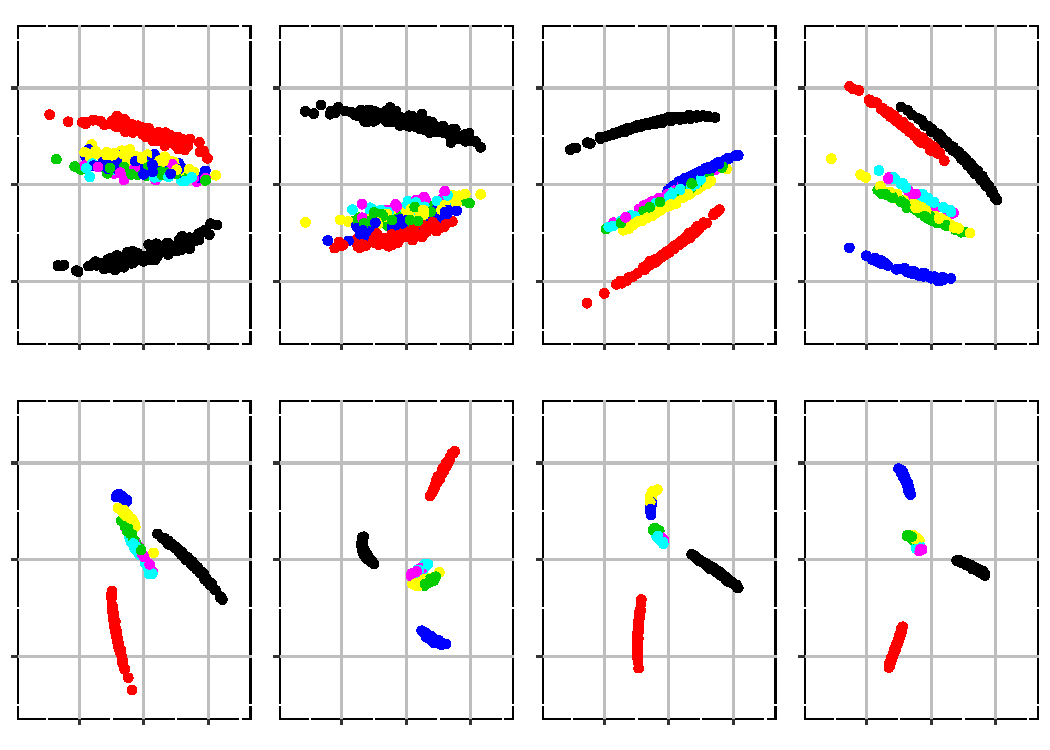
\includegraphics[ width = 0.8\textwidth]{Figs/pca.pdf}
  \caption{first two principal components of transcripts under different parameters for simulated data. Different parameters resulted in different degree of separation of subtypes. We have 4 different settings for hyper-parameters of simulation, each setting has 2 replicates}
  \label{fig:4}
\end{figure}



\noindent
{\bf Data sets}


\begin{table}[ht]
\small
\centering
\begin{tabular}{ |p{3cm}|p{5cm}|p{3cm}|p{2cm}|p{1cm}|}
\hline
 Data set & Conditions & Number of cells/condition & Organism  & Ref\\ \hline \hline
GSE52529 & T0 vs T24 & 96,96 & human & \cite{Trapnell}\\ \hline
GSE57872 & patient1 vs patient2 & 192,96 & human & \cite{Patel} \\ \hline
GSE48968-GPL13112 & BMDC (2h LPS stimulation) vs 6h LPS & 96,96 & mouse & \cite{Shalek} \\ \hline
GSE60749-GPL13112 & serum + LIF vs  2i + LIF & 90,94 & mouse & \cite{Kumar} \\ \hline
GSE74596 & NKT1 vs NTK2 & 46,68 & mouse & \cite{Engel}\\ \hline
EMTAB2805 & G1 vs G2M & 96,96 & mouse & \cite{EMTAB}\\ \hline
GSE71585-GPL13112 &Gad2tdTpositive vs Cux2tdTnegative  & 80,140 & mouse & \cite{Tasic} \\ \hline
GSE64016 & G1 vs G2 & 91,76 & human & \cite{oscope} \\ \hline
GSE79102 & patient1 vs patient2 & 51, 89 & human & \cite{sc3} \\ \hline
GSE45719 & 16-cell stage blastomere vs mid blastocyst cell & 50, 60 & mouse & \cite{Deng193}\\ \hline
GSE63818 & Primordial Germ Cells, develop- mental stage: 7 week gestation vs Somatic Cells, developmental stage: 7 week gestation & 40,26 & mouse & \cite{Guo}\\ \hline
GSE75748 & DEC vs EC & 64, 64 & human & \cite{chu}\\ \hline
GSE84465 & neoplastic cells vs non-neoplastic cells & 546, 664 & human & \cite{Darmanis}\\ \hline
\end{tabular}
\captionof{table}{datasets used for comparisons of DD analysis under different methods}
\end{table}







\noindent
{\bf EBSeq}

Suppose we have $K$ subtypes, let $X_g^I = X_{g, 1}^I, ... , X_{g, S_1}^I$ denote transcripts at gene $g$ from subtype $I, I = 1, ... K$.  In the EBSeq model it assumed that counts within subtype $I$ are distributed as Negative Binomial:
$X_{g, s}^I | r_{g,s}, q_g^I \sim NB(r_{g,s}, q_g^I)$ Where

\begin{eqnarray*}
P(X_{g,s}^I | r_{g,s}, q_g^I ) = {X_{g,s} + r_{g,s} - 1 \choose X_{g,s} }(1 - q_g^I)^{X_{g,s}^I} (q_g^I)^{r_{g,s}}
\end{eqnarray*}
and $\mu_{g,s}^I = r_{g,s}(1 - q_g^I) / q_g^I; \sigma_{g,s}^I = r_{g,s}(1 - q_g^I)/ (q_g^I)^2.$

The EBSeq model assumed a prior distribution on $q_g^I : q_g^I | \alpha, \beta^{I_g} \sim Beta(\alpha, \beta^{I_g}).$ The hyperparameter $\alpha$ is shared by all the isoforms and $\beta^{I_g}$ is $I_g$ specific. We further assume that $r_{g,s} = r_{g,0}*l_s$ where $r_{g,0}$ is an isoform specific parameter common across subtypes and $r_{g,s}$ depends on it through the sample-specific normalization factor $l_s$ 

What we are interested at those $K$ groups comparison is the expression pattern, through EBSeq modeling we are able to obtain posterior probabilities over 

\begin{eqnarray*}
M_{g,\pi} = \{ \theta \in \Theta: \; \mu_{g,k} = \mu_{g,k'} \iff k,k' \in b, b \in \pi \}.
\end{eqnarray*}

For any partition $\pi$ of $K$ elements. 

For example $K = 3$, there are 5 expression pattern, $P_1, P_2, ..., P_5$ 

\begin{align*}
&P1: q_g^1 = q_g^2 = q_g^3\\
&P2: q_g^1 = q_g^2 \neq q_g^3\\
&P3: q_g^1 \neq q_g^2 = q_g^3\\
&P4: q_g^1 = q_g^3 \neq q_g^2\\
&P5: q_g^1 \neq q_g^2 \neq q_g^3 \text{ and } q_g^1 \neq q_g^3
\end{align*}

Under the assumption that two groups $I$ and $J$ share the same $q_g$ we can pool the counts from the two groups by viewing them come from same distribution i.e. $X_g^{I, J} | r_{g,s}, q_g \sim NB(r_{g,s}, q_g)$, $q_g | \alpha, \beta^{I_g} \sim Beta(\alpha, \beta^{I_g})$ and obtained the prior predictive function $f_0^{I_g}(X_g^{I,J}) = \int_0 ^1 P(X_g^{I,J} | r_{g,s}, q_g) * P(q_g | \alpha, \beta^{I_g}) dq_g = \Big[ \overset{S}{\underset{s = 1}{\prod}} {X_{g,s} + r_{g,s} - 1 \choose X_{g,s}} \Big] \frac{Beta(\alpha + \Sigma_{s = 1}^S r_{g,s}, \beta^{I_g} + \Sigma_{s = 1}^S X_{g,s})}{Beta(\alpha, \beta^{I_g})}$.  Consequently, we have prior predictive function for $P1, ..., P5$ as

\begin{align*}
&g_1^{I_g}(X_g^{1,2,3}) = f_0^{I_g}(X_g^{1,2,3})\\
&g_2^{I_g}(X_g^{1,2,3}) = f_0^{I_g}(X_g^{1,2})f_0^{I_g}(X_g^3)\\
&g_3^{I_g}(X_g^{1,2,3}) = f_0^{I_g}(X_g^1)f_0^{I_g}(X_g^{2,3})\\
&g_4^{I_g}(X_g^{1,2,3}) = f_0^{I_g}(X_g^{1,3})f_0^{I_g}(X_g^2)\\
&g_5^{I_g}(X_g^{1,2,3}) = f_0^{I_g}(X_g^1)f_0^{I_g}(X_g^2)f_0^{I_g}(X_g^3)\\
\end{align*}

Then the marginal distribution of counts $X_g^{1,2,3}$ is $\overset{5}{\underset{k = 1}{\Sigma}} p_k g_k^{I_g}(X_g^{1,2,3})$, where proportion parameters $p_k$ satisfying $\overset{5}{\underset{k = 1}{\Sigma}} p_k = 1$ and are estimated by EM algorithm. Thus, the posterior probability of an expression pattern $k$ is obtained by:
\begin{eqnarray*}
\frac{p_k g_k(X_g^{1,2,3})}{\overset{5}{\underset{k = 1}{\Sigma}} p_k g_k^{I_g}(X_g^{1,2,3})}
\end{eqnarray*}


\noindent 
{\bf modalclust}


{Product Partition Model}
Let $X = (X_1, X_2, ...,X_n)$ be $n$ one dimension observed data, given a partition for the data $\pi = \{S_1, ..., S_q\}$, where $S_i$ are disjoint subsets of $\{1,2,...,n\}$ and $\bigcup_{i = 1}^{q} S_i = \{1,2,...,n\}$. The likelihood for $X$ satisfying such partition is 
\begin{eqnarray*}
p(X|\pi) = \overset{q}{\underset{i = 1}{\prod}}f(X_{S_i})
\end{eqnarray*}

where $X_{S_i}$ is the vector of observations corresponding to the items of component $S_i$, The component likelihood $f(X_{S})$ is defined for any non-empty component $S$ and can take any form. The partition $\pi$ is the only parameter we are interested at. 
Any other parameters that may have been involved in the model have been integrated over their prior.

The prior distribution for a partition $\pi$ is also taken as a product form. We use the partition that maximize the posterior $p(\pi | X) \propto p(X|\pi) p(\pi)$ as the estimated clustering of $X$.

Dahl demonstrated by some choice of $f$ and prior of $\pi$, we can reduce the time complexity of finding the MAP partition from factorial($n$) to $O(n^2)$ \cite{ref:dahl},  
And the crucial condition for $f$ is that if $X_{S_1}$ and $X_{S_2}$ are overlapped in the sense that  min$\{X_{S_2}\}  <$ max$\{X_{S_1}\}  <$ max$\{X_{S_2}\}$ or min$\{X_{S_1}\}  <$ max$\{X_{S_2}\}  <$ max$\{X_{S_1}\}$, $X_{S_1^*} and X_{S_2^*}$ be the sets of swapping one pair of those overlapped terms and keep the other unchanged. Then $f(X_{S_1}) f(X_{S_2}) \leq f(X_{S_1^*}) f(X_{S_2^*})$. Under such condition, we know that possible MAP candidates must be those partition that for any two subgroups of data, all the data from subgroup1 has to be either greater or smaller than all the data from subgroup2.


In Poisson-Gamma Model we assuming:

\begin{align*}
X_i | \pi, \lambda &\sim Poisson(X_i | \lambda_1\textbf{I}\{i\in S_1\} + ... + \lambda_q\textbf{I}\{i \in S_q\})\\
\pi &\sim p(\pi)\\
\lambda_j &\sim Gamma(\alpha_0, \beta_0)
\end{align*}

where $p(\pi)\propto \overset{q}{\underset{i = 1}{\prod}}\eta_0\Gamma(|S_i|)$. Integrate out $\lambda$, $f(X_{S})$ is obtained as:

\begin{eqnarray*}
f(X_{S}) = \frac{\beta^\alpha}{(|S| + \beta)^{\underset{i \in S}{\Sigma} X_i + \alpha}} \frac{\Gamma(\underset{i \in S}{\Sigma} X_i  + \alpha)}{\Gamma(\alpha)} \frac{1}{\underset{i \in S}{\prod }X_i}
\end{eqnarray*}

$f(X_S)$ still satisfying the condition mentioned

\begin{proof}
if $X_{S_1}$ and $X_{S_2}$ are overlapped, without loss of generality, we assume min$\{X_{S_2}\}  <$ max$\{X_{S_1}\}  <$ max$\{X_{S_2}\}$, and we swap max$\{X_{S_1}\}$ with min$\{X_{S_2}\}$ and keep the rest unchanged or we could also swap max$\{X_{S_1}\}$ with max$\{X_{S_2}\}$. We denote the new set forming by swap of max$\{X_{S_1}\}$ with min$\{X_{S_2}\}$  as $S_1^*$ and $S_2^*$ and swap of max$\{X_{S_1}\}$ with max$\{X_{S_2}\}$ as $S_1^{**}, S_2^{**}$ accordingly. 

Then we need to show  at least one of the following happens 
\begin{align}
&f(X_{S_1^*}) f(X_{S_2^*}) \geq f(X_{S_1}) f(X_{S_2})\\
&f(X_{S_1^{**}}) f(X_{S_2^{**}}) \geq f(X_{S_1}) f(X_{S_2})
\end{align}


Let $a =$ max$\{X_{S_1}\}$, $b = $ min$\{X_{S_2}\}$ and $c = $ max$\{X_{S_2}\}$. $h_1 = \underset{i \in S_1}{\Sigma} X_i - a$ and $h_2 = \underset{i \in S_2}{\Sigma} X_i - b$, $n_1$ and $n_2$ are the number of elements in $S_1$ and $S_2$. Then 
\begin{align*}
f(X_{S_1^*}) f(X_{S_2^*}) &\geq f(X_{S_1}) f(X_{S_2})\\
&\iff\\
\frac{\Gamma(h_1 + a + \alpha)}{(n_1 + \beta)^{h_1 + a +\alpha}} \frac{\Gamma(h_2 + b + \alpha)}{(n_2 + \beta)^{h_2 + b + \alpha}} &\leq \frac{\Gamma(h_2 + a + \alpha)}{(n_2 + \beta)^{h_2+ a +\alpha}} \frac{\Gamma(h_1 + b + \alpha)}{(n_2 + \beta)^{h_1 + b + \alpha}}\\
&\iff\\
\frac{\Gamma(h_1 + a + \alpha)}{\Gamma(h_1 + b + \alpha)} \frac{\Gamma(h_2 + b + \alpha)}{\Gamma(h_2 + a + \alpha)} &\leq (\frac{n_1 + \beta}{n_2 + \beta})^{a - b} \\
\end{align*}

Left hand side of above formula is $\text{LHS}_1 = \frac{(h_1 + b + \alpha)...(h_1 + a - 1 + \alpha)}{(h_2 + b + \alpha) ... (h_2 + a - 1 + \alpha)}$ by the property of Gamma function and $X_i$ are integer.

Similarly,
\begin{align*}
f(X_{S_1^{**}}) f(X_{S_2^{**}}) &\geq f(X_{S_1}) f(X_{S_2})\\
&\iff\\
\frac{\Gamma(h_2 + c + \alpha)}{\Gamma(h_2 + a + \alpha)} \frac{\Gamma(h_1 + a + \alpha)}{\Gamma(h_1 + c + \alpha)} &\leq (\frac{n_2 + \beta}{n_1 + \beta})^{c - a} \\
\end{align*}

 Left hand side of above formula is $\text{LHS}_2 = \frac{(h_2 + a + \alpha)...(h_2 + c - 1 + \alpha)}{(h_1 + a + \alpha) ... (h_1 + c - 1 + \alpha)}$
 
If $h_1 \leq h_2$, then $\text{LHS}_1 \leq (\frac{h_1 + a - 1 + \alpha}{h_2 + a  - 1 + \alpha})^{a - b}$ and $\text{LHS}_2 \leq (\frac{h_2 + c - 1 + \alpha}{h_1 + c  - 1 + \alpha})^{a - b}$

So if $\frac{h_1 + a - 1 + \alpha}{h_2 + a  - 1 + \alpha} \leq \frac{n_1 + \beta}{n_2 + \beta} $ then (12) holds, if $\frac{h_2 + c - 1 + \alpha}{h_1 + c  - 1 + \alpha} \leq \frac{n_1 + \beta}{n_2 + \beta}$ then (13) holds

We multiply those two inequalities, we found that $\frac{h_1 + a - 1 + \alpha}{h_2 + a  - 1 + \alpha} * \frac{h_2 + c - 1 + \alpha}{h_1 + c  - 1 + \alpha} = \frac{h_1 + a - 1 + \alpha}{h_1 + c  - 1 + \alpha} * \frac{h_2 + c - 1 + \alpha}{h_2 + a  - 1 + \alpha} \leq 1$ as $c > a$ and $h_1 \leq h_2$ But $\frac{n_1 + \beta}{n_2 + \beta} * \frac{n_1 + \beta}{n_2 + \beta} = 1$. At least one equality holds, consequently at least one of (12) and (13) holds.

Similar proof for the case $h_1 > h_2$. 





\end{proof}

\noindent
{\bf Randomized k-means}

We random generate one-dimensional data $X$ from a mixture of 5 normal distributions with different means and same variance. We compare clustering results between random weighting and bayesian clustering with Dirichlet process as prior in terms of posterior probabilities that two elements belong to the same class given the whole data and adjusted rand index comparing to the underlying true class label (Fig 12). 

\begin{figure}[h]
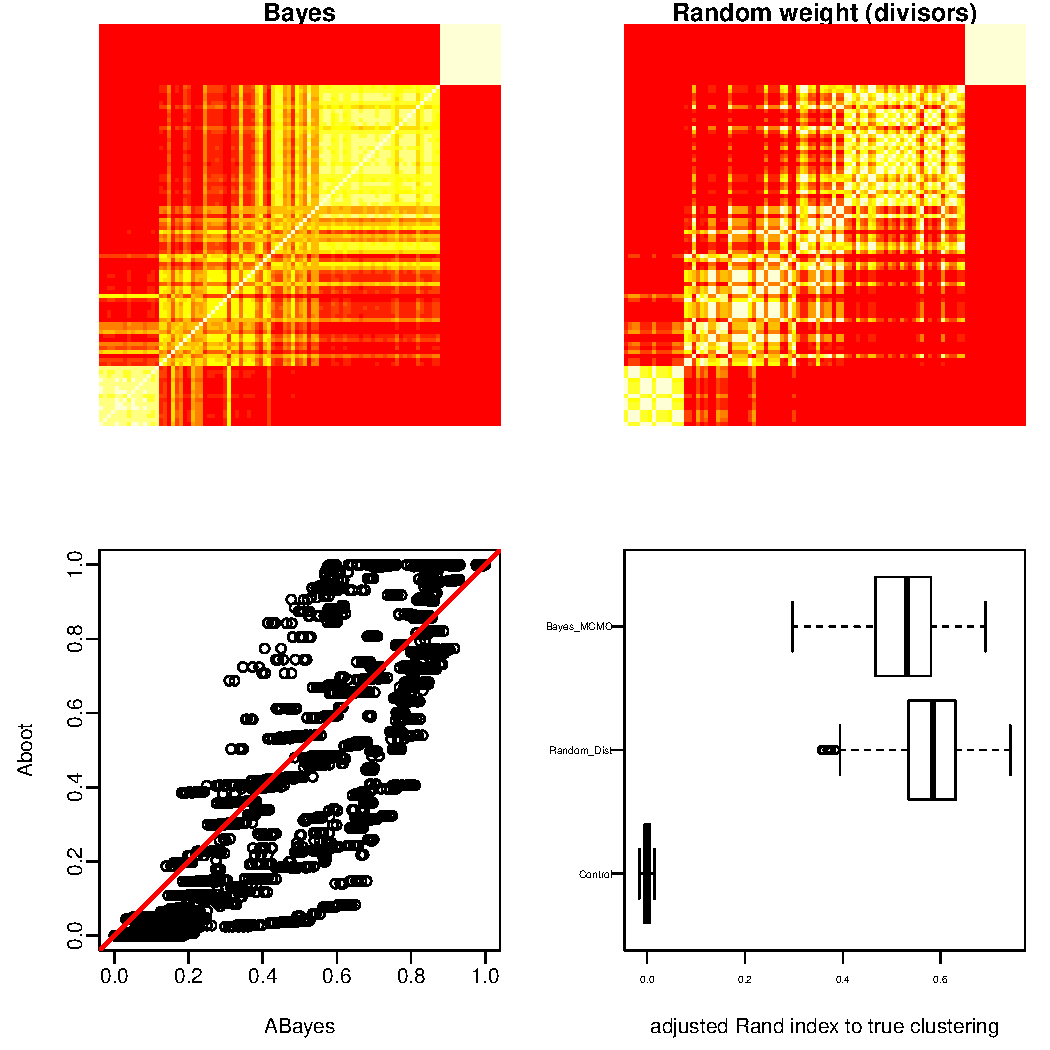
\includegraphics[scale = 1]{Figs/try7-g.pdf}
 \caption{comparison between random weighting scheme and bayesian clustering procedure in terms of posterior probabilities that two elements belong to the same class given the whole data and adjusted rand index comparing to the underlying true class label}
  \label{fig:1}
\end{figure}




\noindent
{\bf Double Dirichlet Model:}

On the double Dirichlet masses, using notation as in Section 2.3 we have density functions:


\begin{eqnarray*}
p_\pi(\phi,\psi) =
         q_\pi( \Phi_\pi, \Psi_\pi  ) \, \prod_{b \in \pi}  \left[
         p( \tilde \phi_b ) p( \tilde \psi_b ) \right]
\end{eqnarray*}
with
\begin{eqnarray*}
q_\pi( \Phi_\pi, \Psi_\pi  )
= \frac{\Gamma(\sum_{b\in \pi} \beta_b)}{
 \prod_{b \in \pi} \Gamma( \beta_b )} \left[\prod_{b \in \pi} \Phi_b^{\beta_b-1} \right] \,
 1\left[ \Phi_\pi = \Psi_\pi \right]
\end{eqnarray*}
and
\begin{eqnarray*}
p( \tilde \phi_b ) =
\frac{ \Gamma( \sum_{k\in b} \alpha_k ) }{ \prod_{k\in b} \Gamma(\alpha_k) }
 \prod_{k \in b} \tilde \phi_k^{\alpha_k -1 },
\qquad
p( \tilde \psi_b )
=
\frac{ \Gamma( \sum_{k\in b} \alpha_k ) }{ \prod_{k\in b} \Gamma(\alpha_k) }
\prod_{k \in b} \tilde \psi_k^{\alpha_k -1 }.
\end{eqnarray*}




\noindent
{\bf Proofs:}


\begin{lemma}
If $\pi_2$ is not refinement of $\pi_1$ then $A_{\pi_1} \cap A_{\pi_2}$ is a lower dimensional subset of $A_{\pi_2}$
\end{lemma}
Proof of theorem 2
\begin{proof}
by lemma 1, it is easy to verify.
\end{proof}
where $p(t^1,t^2|\phi,\psi) = p(t^1|\phi)p(t^1|\psi)$, $t^1|\phi \sim \text{multinomial}(n_1, \phi), t^2|\psi \sim \text{multinomial}(n_2, \psi)$. Recall the definition of $A_\pi = \{(\phi,\psi): \Phi_b = \Psi_b\}$ and $A_\pi$ is a simplex. Denote the finest partition as $\pi_{F} = \{ \{1\}, \{2\},...,\{K\}\}$, associated simplex $A_{\pi_{F}} = \{(\phi, \psi): \phi_i = \psi_i, i = 1,...,K\}$ for any two partition $\pi_1$ and $\pi_2$, intersection of their associated simplex must not be empty since $A_{\pi_{F}}\subset A_{\pi_1}\cap A_{\pi_2} \neq \emptyset$.  To discuss the issue of overlapping of simplex $A_\pi$, we first introduce some notations. The whole space $\Omega = \{ (\phi,\psi), \phi_i,\psi_i > 0 \text{ and } \sum_{i=1}^K \phi_i = \sum_{i=1}^K \psi_i = 1\}$ and we define the refinement and coarseness relationship between partitions, we say a partition $\tilde{\pi}$ refines another partition $\pi$ if $\forall b \in \pi$ there exists $s \subset \tilde{\pi}$  such that $\cup_{b'\in s} b' = b$. When $\tilde{\pi}$ refines $\pi$, we say $\tilde{\pi}$ is a refinement of(finer than) $\pi$ or $\pi$ is a coarseness of(coarser than) $\tilde{\pi}$. 
Observe that if $\pi'$ refines $\pi$, then $A_\pi \cap A_{\pi'} = A_{\pi'}$, $\int_{A_\pi\cap A_{\pi'}} p(z^1,z^2|\phi,\psi)p(\phi, \psi | A_{\pi'})d\phi d\psi = \int_{A_{\pi'}} p(t^1,t^2|\phi,\psi)p(\phi, \psi | A_{\pi'})d\phi d\psi $. When $\pi'$ is not refinement of $\pi$, we need to know the dimension of $A_\pi\cap A_{\pi'}$. Consider a map $f: b \rightarrow v$, which maps the block $b$ to a vector $v\in \{0, 1\}^K$, the ith component of $v$ is $1_{\{i\in b\}}$. And denote $\text{dim}(S)$ be the dimension of space $S$. $A_\pi$ can be equivalently defined as $A_\pi =  \{(\phi,\psi): M_\pi * (\phi - \psi) = 0\}$, $M_\pi$ is a matrix with rows be $v_b = f(b), \forall b\in \pi$, that is to say $(\phi,\psi)$ are in the null space of linear transformation $M_\pi$.  We have following lemma\\
Proof of lemma 1
\begin{proof}
Let $V$ denote the orthogonal space of $\phi - \psi$, when $(\phi,\psi)\in A_{\pi_1} \cap A_{\pi_2}$, and $\text{dim}(A_{\pi_1} \cap A_{\pi_2}) = \text{dim}(\phi - \psi) + \text{dim}(\psi) = 2K - \text{dim}(V) - 1$. Also let $\pi_1 = \{b_1^1,...,b_s^1\}, \pi_2 = \{b_1^2,...,b_t^2\}$. The corresponding vectors are $v_1^1,...,v_s^1$ and $v_1^2,...,v_t^2$. We claim there must be a $b_i^1\in \pi$ whose corresponding $v_i^1$ is linear independent with $v_1^2,...,v_t^2$. If not, for every $v_i^1$ there exists $\alpha_1^i,...,\alpha_t^i$ such that 
\[
v_i^1 = \sum_{j = 1}^t \alpha_j^i v_j^2 \quad\quad\quad(*)
\]
If $b_j^2 \cap b_i^1 \neq \emptyset$, then multiply $v_j^2$ on both sides of (*), we obtain $v_i^1 * v_j^2 = \alpha_j^i (v_j^2)^2$, as $v_j^2$ are orthogonal vectors, and $v_i^1 * v_j^2 > 0$ implies $\alpha_j^i > 0$. Consider $x = f(b_j^2\setminus b_i^1)$, we have $x*v_i^1 = 0$ and we multiply $x$ on both sides of (*) to obtain $\alpha_j^i v_j^2*x = 0$, thus x must be zero vector and $b_j^2\setminus b_i^1= \emptyset$, which implies $b_j^2 \subset b_i^1$. That is to say when $b_j^2 \cap b_i^1 \neq \emptyset$, $b_j^2$ must be subset of $b_i^1$. So $b_i^1$ is union of some blocks in $\pi_2$. Which implies $\pi_2$ is refinement of $\pi_1$, contradiction.\\
Consequently there exists $b\in\pi_1$ with $v(b)$ linear independent with $v(b'), b'\in\pi_2$. $\text{dim}(V)$ is at least $N(\pi_2) + 1, \dim(A_{\pi_1} \cap A_{\pi_2}) < \text{dim}(A_{\pi_2})$
\end{proof}
\hfill\\
Proof of theorem 3 and theorem 4
\begin{proof}
Given the condition that $\alpha_k = 1, \forall k$ and $\beta_b = \sum_{k\in b} \alpha_k$, recall $p(A_\pi| t^1, t^2) = \sum_{\pi' \in \text{RF}(\pi)} J(t^1,t^2,\pi')$  and $J(t^1, t^2 ,\pi) = \frac{1}{c'}\prod_{b\in \pi}\frac{ \Gamma(\beta_b + t_b^1 + t_b^2)}{\Gamma(\beta_b + t_b^1)\Gamma(\beta_b + t_b^2)}$\\
Assuming there are $K$ subgroups, since $n_1$ and $n_2$ goes to infinite at same rate, for simplicity we assume $n = \sum_{i = 1}^K t_i^1 = \sum_{i = 1}^K t_i^2 $,  $t^1\sim \text{multinomial}(\phi), t^2\sim \text{multinomial}(\psi)$ and
$t_b^1 = \sum_{i \in b} z_i^1$ and $t_b^2 = \sum_{i \in b} z_i^2$, so $t_b^1 \sim$ binomial $(n, \Phi_b)$ and $t_b^2 \sim$ binomial $(n, \Psi_b)$, where $\Phi_b = \sum_{i \in b}\phi_i$ and $\Psi_b = \sum_{i \in b}\psi_i$. Let $f(n, b) = \frac{\Gamma(\beta_b + t_b^1 + t_b^2)}{\Gamma(\beta_b + t_b^1)\Gamma(\beta_b + t_b^2)}$, then 
$$J(z^1, z^2 ,\pi) \propto \prod_{b\in \pi} f(n,b)$$\\
log$f(n, b) = $log$(\Gamma(\beta_b + t_b^1 + t_b^2))$ - log$(\Gamma(\beta_b + t_b^1))$ - log$(\Gamma(\beta_b + t_b^2))$, notice that $t_b^1, t_b^2 \text{ and } \beta_b$ are integers, and when $x$ is integer,  $\Gamma(x)$ is the factorial of $(x - 1)$.
We have log$f(n, b) = $log$((\beta_b + t_b^1 + t_b^2 -1)!) - \text{log}((\beta_b + t_b^1 -1)!) - \text{log}((\beta_b + t_b^2 -1)!)$  and when $n$ is large we could use Stirling's approximation, i.e. log$(n!)$ = $n$log$(n) - n + O(\text{log}(n))$, we have log$((\beta_b + t_b^1 + t_b^2 -1)!) - \text{log}((\beta_b + t_b^1 -1)!) - \text{log}((\beta_b + t_b^2 -1)!)\approx (\beta_b + t_b^1 + t_b^2-1)\text{log}(\beta_b + t_b^1 + t_b^2-1) - (\beta_b + t_b^1 -1)\text{log}(\beta_b + t_b^1 -1) - (\beta_b + t_b^2 -1)\text{log}(\beta_b + t_b^2 -1) + O(\text{log}(n))$.\\
Plug into $f(n,b)$ we have:\\
$$\text{log}f(n,b) \approx (\beta_b + t_b^1 -1)\text{log}(1 + \frac{t_b^2}{\beta_b + t_b^1 -1}) + (\beta_b + t_b^2 -1)\text{log}(1 + \frac{t_b^1}{\beta_b + t_b^2 -1}) + O(\text{log}(n))$$\\
as $\beta_b \text{log}(\beta_b + t_b^1 + t_b^2 -1) \sim O(\text{log}(n))$ and by law of large number and slutsky's theorem, $\text{log}(1 + \frac{t_b^2}{\beta_b + t_b^1 -1}) \rightarrow \text{log}(1+\frac{\Psi_b}{\Phi_b})$,
$\text{log}(1 + \frac{t_b^1}{\beta_b + t_b^2 -1}) \rightarrow \text{log}(1+\frac{\Phi_b}{\Psi_b})$ $a.s.$ and $\frac{\text{log}f(n, b)}{n} \rightarrow \Phi_b\text{log}(1+\frac{\Psi_b}{\Phi_b}) + \Psi_b\text{log}(1+\frac{\Phi_b}{\Psi_b})$ a.s. We have:\\
$$ \frac{\text{log}(\prod_{b\in \pi} f(n,b))}{n} \rightarrow \sum_b [\Phi_b\text{log}(1+\frac{\Psi_b}{\Phi_b}) + \Psi_b\text{log}(1+\frac{\Phi_b}{\Psi_b})] \quad a.s.$$
To find the maxima $(\Phi, \Psi)$, we fix $\Psi$ and 
let $C =  \frac{\text{log}(\prod_{b\in \pi} f(n,b))}{n} + \lambda(\underset{b\in\pi}\sum \Phi_b - 1)$, we have $\frac{\partial C}{\partial \Phi_b} =  \text{log}(1+\frac{\Psi_b}{\Phi_b}) + \lambda$, stationary point is $\Phi_b = \Psi_b, \forall b$. and for the hessian matrix $\frac{\partial^2 C}{\partial \Phi_b^2} = -\frac{\Psi_b}{\Phi_b^2 + \Phi_b\Psi_b} < 0$ and $\frac{\partial^2 C}{\partial \Phi_{b}\partial \Phi_{b'}} = 0, \text{if } b \neq b'$, that is to say the hessian matrix is a diagonal matrix with every diagonal elements to be negative, so it is negative definite, and our objective function is concave. The maxima is the stationary point $\Phi = \Psi$. 
And when $\Phi = \Psi$ , $\frac{\text{log}(\prod_{b\in \pi} f(n,b))}{n} = 2\text{ln}(2)$ a constant not dependent on partition $\pi$ and $\Phi$. That is to say if $(\phi,\psi) \in A_{\pi_1}\cap A_{\pi_2}$ and $(\phi,\psi) \notin A_{\pi_3}$. Then we would have 
$\lim_{n\to\infty}\frac{\text{log}(\prod_{b\in \pi_1} f(n,b))}{n} = \lim_{n\to\infty}\frac{\text{log}(\prod_{b\in \pi_2} f(n,b))}{n}$ and  $\lim_{n\to\infty}[\frac{\text{ln}(\prod_{b\in \pi_1} f(n,b))}{n} -  \frac{\text{log}(\prod_{b\in \pi_3} f(n,b))}{n}]  = c > 0 $, which implies:
\[\frac{J(t^1, t^2,\pi_3)}{J(t^1, t^2,\pi_1)} \rightarrow 0\quad a.s. \tag{A}\]
To investigate the limit of $\frac{J(t^1, t^2,\pi_1)}{J(t^1, t^2,\pi_2)}$, We use inequalities that $\sqrt{2\pi}n^{n+\frac{1}{2}}e^{-n} \leq n! \leq en^{n+\frac{1}{2}}e^{-n}$ holds for all nonnegative integers $n$. Plug in $f(n,b)$, we have:\\
\[
\beta_b +\text{log}\sqrt{2\pi} - 3 + g(n,b) 
\leq f(n, b)\leq
\beta_b - 2\text{log}\sqrt{2\pi} + g(n, b)\tag{1}
\]\\
\[g(n,b) =  (\beta_b + t_b^1 - \frac{1}{2})\text{log}(1 + \frac{t_b^2}{\beta_b + t_b^1 -1}) + (\beta_b + t_b^2 - \frac{1}{2})\text{log}(1 + \frac{t_b^1}{\beta_b + t_b^2 -1}) - (\beta_b - \frac{1}{2})\text{log}(\beta_b + t_b^1 + t_b^2 - 1)\]\\
Based on inequalities (1), $\underset{{b\in\pi}}\sum f(n,b)$ only differ with $\underset{b\in\pi}\sum g(n,b)$ by a constant.
By Taylor's expansion $\text{log}(1+x) = \text{log}2 + \frac{1}{2}(x - 1) + O( (x-1)^2)$, we have $\text{log}(1 + \frac{t_b^2}{\beta_b + t_b^1 -1}) = \text{log}2 + \frac{1}{2}(\frac{t_b^1 - t_b^2 + 1 - \beta_b}{\beta_b + t_b^1 -1}) + O_p((\frac{t_b^1 - t_b^2 + 1 - \beta_b}{\beta_b + t_b^1 -1})^2)$ and under condition $\Phi_b = \Psi_b, \frac{(t_b^1 - t_b^2 + 1 - \beta_b)^2}{\beta_b + t_b^1 -1}$ is $O_p(1)$. Plug in $g(n,b)$\\
$$g(n,b) = \text{log}2 * t_b^1 + \text{log}2 * t_b^2  - (\beta_b - \frac{1}{2})\text{log}(\beta_b + t_b^1 + t_b^2 - 1) + O_p(1) $$
and sum up 
\[\sum_{b\in\pi} g(n,b) = 2n\text{log}2 - \sum_{b\in\pi}(\beta_b - \frac{1}{2})\text{log}(\beta_b + t_b^1 + t_b^2 - 1) + O_p(1)  \tag{2} \]
Notice that when two partition $\pi_1$, $\pi_2$ have same number of blocks $b$ and $\Phi_b = \Psi_b$, $\forall b \in \pi_1\cup\pi_2$, 
\begin{align*}
\sum_{b\in\pi_1} g(n,b) - \sum_{b'\in\pi_2} g(n,b') &= \sum_{b'\in\pi_2}(\beta_b' - \frac{1}{2})\text{log}(\beta_b' + t_{b'}^1 + t_{b'}^2 - 1) - \sum_{b\in\pi_1}(\beta_b - \frac{1}{2})\text{log}(\beta_b + t_b^1 + t_b^2 - 1) +  O_p(1)\\
&= \sum_{b'\in\pi_2}(\beta_{b'}- \frac{1}{2})\text{log}(\frac{\beta_b' + t_{b'}^1 + t_{b'}^2 - 1}{n}) -  \sum_{b\in\pi_1}(\beta_b - \frac{1}{2})\text{log}(\frac{\beta_b + t_b^1 + t_b^2 - 1}{n})\\
 &+ \sum_{b'\in\pi_2 - \frac{1}{2}}(\beta_{b'}  - \frac{1}{2})\text{log}(n) - \sum_{b\in\pi_1 - \frac{1}{2}}(\beta_b - \frac{1}{2})\text{log}(n) + O_p(1)\\
&= O_p(1) + \sum_{b\in\pi_1}\frac{1}{2}\text{log}(n) - \sum_{b'\in\pi_2}\frac{1}{2}\text{log}(n) \\
&= O_p(1)
\end{align*}
When $\pi_1$ and $\pi_2$ have same number of blocks,  
\[\frac{J(t^1, t^2,\pi_1)}{J(t^1, t^2,\pi_2)} \rightarrow O_p(1)\quad a.s. \tag{B}\]
When $\pi_1$ have less blocks than $\pi_2$, $\sum_{b'\in\pi_2} g(n,b') - \sum_{b\in\pi_1} g(n,b) = O_p(\text{log}(n))$
\[\frac{J(t^1, t^2,\pi_1)}{J(t^1, t^2,\pi_2)} \rightarrow 0\quad a.s.\tag{C}\]
\end{proof}



\end{document}  
